\documentclass[11pt,a4paper]{article}
\usepackage[T1]{fontenc}\usepackage[utf8]{inputenc}\usepackage{mathptmx,courier,microtype}
\usepackage[margin=24mm]{geometry}\usepackage{amsmath,amssymb,booktabs,tabularx,longtable,graphicx}
\usepackage[obeyspaces]{url}\usepackage{hyperref}\usepackage{tikz}
\usetikzlibrary{arrows.meta,positioning}\hypersetup{hidelinks}
\setlength{\parindent}{0pt}\setlength{\parskip}{6pt}\setlength{\emergencystretch}{3em}
\newcommand{\plot}[2]{\begin{center}\includegraphics[width=\linewidth]{generated/#1.pdf}\end{center}\noindent\textbf{Figure:} #2}
\begin{document}\begin{center}{\LARGE\bfseries WavLM-Large for Parkinson's\\Speech Classification}\par\vspace{10pt}
{\large Proposal Experiment: Verified Speaker-disjoint OOF Evaluation}\par
Arannamoy Mondal\par 14 October 2026\quad Report 1.0\quad Experiment v4.0\end{center}\hrule
\section*{Abstract}
This separate experiment implements the WavLM-based proposal using the latest
PatchTST technical report's evidence structure. It asks whether Random Forest
or XGBoost improves on logistic regression when all three receive exactly the
same frozen WavLM-large recording embeddings, speech tasks and speaker folds.
It uses 773 recordings from 46 canonical people, 25 with Parkinson's disease
and 21 elderly controls. It does not replace the official v2.0 PatchTST result.
The frozen logistic baseline has pooled speaker F1 97.96\%, recall 96.00\%, specificity 100.00\%, precision 100.00\%, and accuracy 97.83\%.
All comparisons are revised internal evaluations on a previously studied corpus.
Speaker separation and training-side selection are checked, but recording-condition
confounding and external clinical generalization remain unresolved.
\section{One question, one input, three matched classifiers}
The input is a 1,024-value representation of each recording, extracted by a pinned,
frozen WavLM-large encoder. Logistic regression is the predeclared baseline;
Random Forest and XGBoost are extensions, not replacements chosen after looking
at a test score. All three use the same cohort, tasks, outer folds, inner splits,
training weights and threshold. The question concerns corpus-label classification,
not a new clinical diagnosis.
\clearpage\section{The whole pipeline}
\begin{center}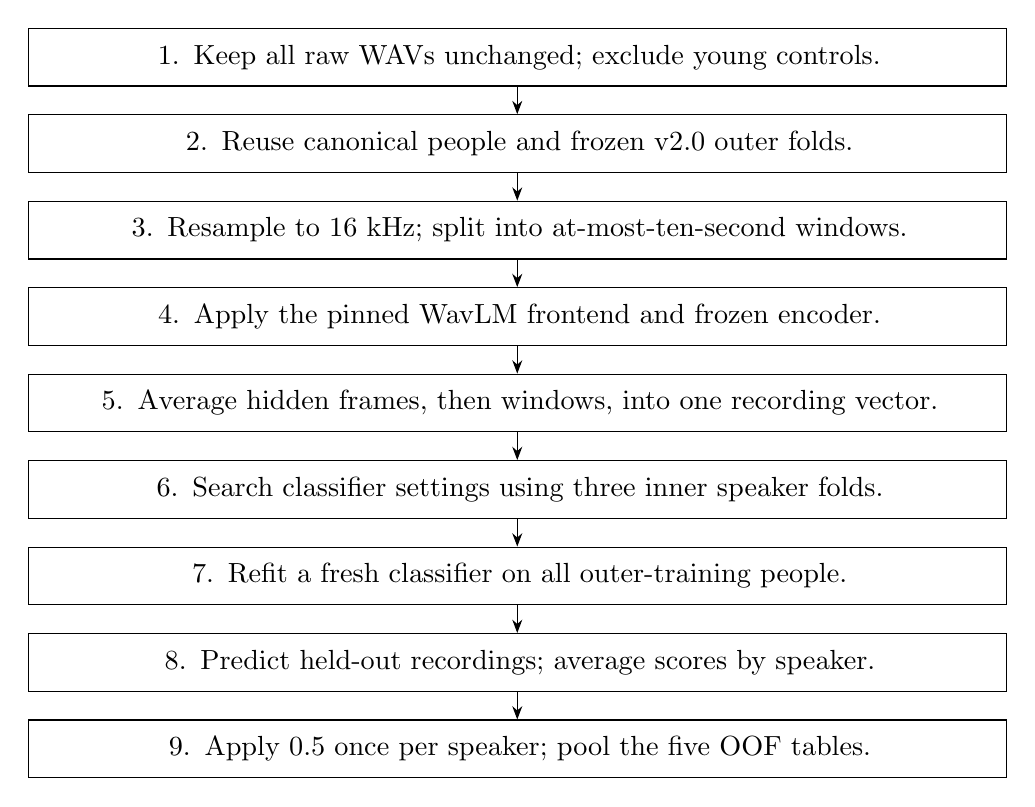
\begin{tikzpicture}[node distance=0.35cm,
box/.style={draw,align=center,text width=12cm,inner sep=6pt},
arr/.style={-{Stealth},draw=black}]
\node[box](a){1. Keep all raw WAVs unchanged; exclude young controls.};
\node[box,below=of a](b){2. Reuse canonical people and frozen v2.0 outer folds.};
\node[box,below=of b](c){3. Resample to 16 kHz; split into at-most-ten-second windows.};
\node[box,below=of c](d){4. Apply the pinned WavLM frontend and frozen encoder.};
\node[box,below=of d](e){5. Average hidden frames, then windows, into one recording vector.};
\node[box,below=of e](f){6. Search classifier settings using three inner speaker folds.};
\node[box,below=of f](g){7. Refit a fresh classifier on all outer-training people.};
\node[box,below=of g](h){8. Predict held-out recordings; average scores by speaker.};
\node[box,below=of h](i){9. Apply 0.5 once per speaker; pool the five OOF tables.};
\foreach \x/\y in {a/b,b/c,c/d,d/e,e/f,f/g,g/h,h/i}\draw[arr](\x)--(\y);
\end{tikzpicture}\end{center}
Fixed feature extraction learns nothing from this corpus. Classifier fitting,
scaling, parameter selection and the optional fine-tuning decision remain inside
training people. Every number reported below is generated from saved predictions.
\clearpage\section{The recordings and canonical people}
The unmodified corpus contains 831 WAV files. Removing 45 young-control files
leaves an eligible 786-recording index with 47 working person identities.
Known repeat sessions for Vito S, Nicola S and Roberto R are linked before splitting.
The study deliberately retains the latest report's common cohort: 773 files and
46 people. Vitantonio D lacks passage recordings and remains excluded from that
shared cohort. This is a design choice, not a requirement of WavLM itself.
Age, sex, CPS, native sample rate, dates, names, tasks and paths are metadata;
none is appended to the classifier feature vector. Task names only describe errors.
Young controls remain outside both training and reported evaluation.
The native-rate sensitivity experiment retains 613 recordings from 39 people:
18 patients and 21 controls. It is retrained separately using only recordings
originally sampled at 16 kHz. Three flagged controls are removed only in the
separate main-OOF sensitivity evaluation; those models are not retrained.
\clearpage\section{From waveform to WavLM representation}
Mono PCM is read as float32 and resampled to 16 kHz with librosa's soxr\_hq.
No extra peak normalization, task trimming or metadata-derived feature is applied.
The pinned pretrained frontend then performs its standard mean/variance
normalization within each waveform window. This is not peak normalization,
but it removes absolute waveform level cues, including some potential voice-level
and recording-gain information. It differs from the level-preserving PatchTST input.
Windows cover at most ten seconds. Long recordings use consecutive ten-second
windows, plus a final overlapping full window when needed to cover the tail.
Short recordings remain short; only inputs below the convolutional minimum of
400 samples are edge-padded. A ten-second window produces 499 hidden frames.
\[
e_{jk}=\frac{1}{T_{jk}}\sum_t h_{jkt}\in\mathbb R^{1024},\qquad
e_j=\frac{1}{K_j}\sum_k e_{jk}.
\]
The encoder has 315,453,120 parameters, all frozen during this extraction.
It has 24 transformer layers, 1,024 hidden values and 16 attention heads.
It is a pretrained speech representation, not 1,024 handcrafted measurements.
Revision: \path{c1423ed94bb01d80a3f5ce5bc39f6026a0f4828c}.
The exact checkpoint, frontend and configuration files are fingerprinted.
WavLM was pretrained for general speech representation; Italian-corpus success
does not demonstrate language-independent or clinical generalization.
\clearpage\section{What each classifier learns}
\textbf{Logistic regression:} a training-fitted weighted standard scaler followed
by regularized linear classification. C is selected from 0.01, 0.1, 1 and 10.
\textbf{Random Forest:} 300 trees; depths 4 or unrestricted; minimum leaves
1 or 2; square-root feature subsampling. No learned scaler is required.
\textbf{XGBoost:} 200 histogram-based boosting rounds; depths 1, 2 or 3;
learning rates 0.03 or 0.1; half of embedding columns considered per tree;
L2 regularization 1. These six settings are predeclared.
The grids contain 4, 4 and 6 candidates respectively. The first candidate in
the frozen grid order wins exact validation-score ties. There is no outer-test
early stopping, threshold search, feature selection or best-fold selection.
Feature values must be finite. Invalid cache files stop the run rather than
silently being imputed or dropped.
\clearpage\section{Nested speaker folds and final refit}
The five outer folds are exactly those of v2.0. Each held-out person receives
a prediction from a model trained without that person. Repeat sessions and
all recordings from a person stay together.
Inside each outer-training group, three stratified inner speaker folds evaluate
every candidate. Each inner model fits only its training people, predicts its
validation recordings, and averages those probabilities to speakers before AUROC
is calculated. The average of the three validation AUROCs chooses the setting.
The selected model is then fitted again from scratch on all outer-training people.
The outer test group never chooses the classifier, hyperparameters or threshold.
Unlike PatchTST's single validation holdout, this experiment has three rotating
training/validation pairs inside each outer fold. The exact 80 partition CSVs
cover both main and native-rate scenarios. Final refit contains all development
people, not only an inner training subset.
\clearpage\section{Equal training influence and speaker decisions}
Each training class receives equal total weight. Within each class, every person
receives equal weight; within a person, every recording receives an equal share.
For recording j from person i in class c, raw weight is
\[
w_{ij}=1/(N_c F_i).
\]
Weights are rescaled to have mean one. The scaler and classifier receive only
current-training rows and weights. Test people never determine these counts.
The classifiers operate on complete recording vectors. A person's final score is
the equal average of that person's recording probabilities, not a pooled average
of every window and not an average of hard class labels.
\[
p_i=\frac{1}{F_i}\sum_j f(e_j),\qquad \hat y_i=\mathbf 1[p_i\geq0.5].
\]
The first averaging stage here combines embeddings before the recording classifier;
the second combines recording probabilities. It is not identical to averaging
PatchTST window probabilities, and the distinction is intentional and recorded.
Each person contributes one OOF row, regardless of recording count or duration.
\clearpage\section{The conditional fine-tuning rule}
The proposal suggests partial fine-tuning when baseline AUROC is below 0.80.
This implementation applies that rule to the selected logistic baseline's mean
inner speaker AUROC separately in each outer fold. Pooled outer-test AUROC never
chooses whether a model is trained.
If triggered, a training-side holdout compares two or four upper layers and learning
rates of $10^{-5}$ or $3\cdot10^{-5}$. Binary cross-entropy selects an epoch count,
with at most six epochs and patience two. Validation AUROC selects the candidate.
The lower encoder stays frozen and deterministic. Training uses at most two windows
per recording; evaluation uses all windows. A fresh pretrained model is refitted
on all outer-training people for the selected epoch count before testing.
0 of the ten main/native outer folds triggered fine-tuning. No upper-layer model was trained in this experiment. The conditional pipeline reuses the frozen logistic baseline and must not be presented as an independent fourth model. The ten training-side gate values range from 0.9921 to 1.0000.
\clearpage\section{Five operating-point metrics and ranking}
F1 compares precision and recall but ignores true negatives. Recall counts detected
patients; specificity counts correctly excluded controls. Precision concerns the
people called positive in this nearly balanced sample. Accuracy counts all correct
decisions. The five are always shown together, in percentages.
Precision in this nearly balanced speaker sample is not community-screening
positive predictive value. Model scores are not established clinical risk probabilities.
AUROC describes ranking across thresholds. Trapezoidal AUPRC integrates the
precision--recall curve; average precision uses a different step-weighted definition
and is reported separately. Neither selects a new threshold after testing.
Fold mean and sample SD describe variation in these five small folds, not a
confidence interval for deployment. The experimental sample is 46 people,
not 773 independent patients. The proposal's above-85\% pooled-F1 target is
assessed as an internal numerical target, not clinical validation.

\clearpage\section{Main result: Logistic regression}
\begin{center}\small\begin{tabular}{lrrrrrr}\toprule Fold & People & F1 & Recall & Specificity & Precision & Accuracy\\\midrule
0 & 10 & 100.00 & 100.00 & 100.00 & 100.00 & 100.00\\
1 & 9 & 100.00 & 100.00 & 100.00 & 100.00 & 100.00\\
2 & 9 & 100.00 & 100.00 & 100.00 & 100.00 & 100.00\\
3 & 9 & 100.00 & 100.00 & 100.00 & 100.00 & 100.00\\
4 & 9 & 88.89 & 80.00 & 100.00 & 100.00 & 88.89\\
Mean/SD & -- & 97.78 $\pm$ 4.97 & 96.00 $\pm$ 8.94 & 100.00 $\pm$ 0.00 & 100.00 $\pm$ 0.00 & 97.78 $\pm$ 4.97\\\midrule
Pooled & 46 & 97.96 & 96.00 & 100.00 & 100.00 & 97.83\\\bottomrule\end{tabular}\end{center}
Pooled confusion counts: TP=24, FN=1, TN=21, FP=0.

AUROC=0.9943; trapezoidal AUPRC=0.9956; average precision=0.9957.

The pooled F1 exceeds the proposal's 85\% numerical target. 
Misclassified people: PD\_CFAERLEI54F (true label 1, score 0.18830).

\clearpage\section{Main result: Random Forest}
\begin{center}\small\begin{tabular}{lrrrrrr}\toprule Fold & People & F1 & Recall & Specificity & Precision & Accuracy\\\midrule
0 & 10 & 100.00 & 100.00 & 100.00 & 100.00 & 100.00\\
1 & 9 & 100.00 & 100.00 & 100.00 & 100.00 & 100.00\\
2 & 9 & 100.00 & 100.00 & 100.00 & 100.00 & 100.00\\
3 & 9 & 100.00 & 100.00 & 100.00 & 100.00 & 100.00\\
4 & 9 & 88.89 & 80.00 & 100.00 & 100.00 & 88.89\\
Mean/SD & -- & 97.78 $\pm$ 4.97 & 96.00 $\pm$ 8.94 & 100.00 $\pm$ 0.00 & 100.00 $\pm$ 0.00 & 97.78 $\pm$ 4.97\\\midrule
Pooled & 46 & 97.96 & 96.00 & 100.00 & 100.00 & 97.83\\\bottomrule\end{tabular}\end{center}
Pooled confusion counts: TP=24, FN=1, TN=21, FP=0.

AUROC=0.9943; trapezoidal AUPRC=0.9956; average precision=0.9957.

The pooled F1 exceeds the proposal's 85\% numerical target. 
Misclassified people: PD\_CFAERLEI54F (true label 1, score 0.33270).

\clearpage\section{Main result: XGBoost}
\begin{center}\small\begin{tabular}{lrrrrrr}\toprule Fold & People & F1 & Recall & Specificity & Precision & Accuracy\\\midrule
0 & 10 & 100.00 & 100.00 & 100.00 & 100.00 & 100.00\\
1 & 9 & 100.00 & 100.00 & 100.00 & 100.00 & 100.00\\
2 & 9 & 100.00 & 100.00 & 100.00 & 100.00 & 100.00\\
3 & 9 & 100.00 & 100.00 & 100.00 & 100.00 & 100.00\\
4 & 9 & 80.00 & 80.00 & 75.00 & 80.00 & 77.78\\
Mean/SD & -- & 96.00 $\pm$ 8.94 & 96.00 $\pm$ 8.94 & 95.00 $\pm$ 11.18 & 96.00 $\pm$ 8.94 & 95.56 $\pm$ 9.94\\\midrule
Pooled & 46 & 96.00 & 96.00 & 95.24 & 96.00 & 95.65\\\bottomrule\end{tabular}\end{center}
Pooled confusion counts: TP=24, FN=1, TN=20, FP=1.

AUROC=0.9848; trapezoidal AUPRC=0.9902; average precision=0.9903.

The pooled F1 exceeds the proposal's 85\% numerical target. 
Misclassified people: EHC\_GCIALSDA52F (true label 0, score 0.53230); PD\_CFAERLEI54F (true label 1, score 0.28048).

\subsection*{Answer to the matched-classifier question}
Random Forest: F1 ties the logistic baseline; AUROC ties the logistic baseline; AUPRC ties the logistic baseline.

XGBoost: F1 is below the logistic baseline; AUROC is below the logistic baseline; AUPRC is below the logistic baseline.

These are descriptive comparisons on the same 46 people, not evidence of a statistically established advantage. A more complex classifier is not automatically an improvement.

The native-rate cohort excludes main-error speaker(s) PD\_CFAERLEI54F. Consequently, its perfect score changes the people evaluated as well as the training data; it is not an independent confirmation on the original cohort.

\clearpage\section{Flag exclusion and native-rate retraining}
\subsection*{Main OOF without flagged controls}
\textbf{Logistic regression}\begin{center}\small\begin{tabular}{lrrrrrr}\toprule Fold & People & F1 & Recall & Specificity & Precision & Accuracy\\\midrule
Pooled & 43 & 97.96 & 96.00 & 100.00 & 100.00 & 97.67\\\bottomrule\end{tabular}\end{center}
\textbf{Random Forest}\begin{center}\small\begin{tabular}{lrrrrrr}\toprule Fold & People & F1 & Recall & Specificity & Precision & Accuracy\\\midrule
Pooled & 43 & 97.96 & 96.00 & 100.00 & 100.00 & 97.67\\\bottomrule\end{tabular}\end{center}
\textbf{XGBoost}\begin{center}\small\begin{tabular}{lrrrrrr}\toprule Fold & People & F1 & Recall & Specificity & Precision & Accuracy\\\midrule
Pooled & 43 & 97.96 & 96.00 & 100.00 & 100.00 & 97.67\\\bottomrule\end{tabular}\end{center}
\subsection*{Native-16-kHz-only retraining}
\textbf{Logistic regression}\begin{center}\small\begin{tabular}{lrrrrrr}\toprule Fold & People & F1 & Recall & Specificity & Precision & Accuracy\\\midrule
Pooled & 39 & 100.00 & 100.00 & 100.00 & 100.00 & 100.00\\\bottomrule\end{tabular}\end{center}
\textbf{Random Forest}\begin{center}\small\begin{tabular}{lrrrrrr}\toprule Fold & People & F1 & Recall & Specificity & Precision & Accuracy\\\midrule
Pooled & 39 & 100.00 & 100.00 & 100.00 & 100.00 & 100.00\\\bottomrule\end{tabular}\end{center}
\textbf{XGBoost}\begin{center}\small\begin{tabular}{lrrrrrr}\toprule Fold & People & F1 & Recall & Specificity & Precision & Accuracy\\\midrule
Pooled & 39 & 100.00 & 100.00 & 100.00 & 100.00 & 100.00\\\bottomrule\end{tabular}\end{center}
Flag exclusion changes evaluation people only, not fitted models. Native-rate restriction genuinely retrains all models, but also changes the patient cohort. It is not independent confirmation and does not match microphones, rooms or recruitment conditions.

\clearpage\section{Exact partition sizes}
\begin{center}\small\begin{tabular}{lrrrr}\toprule Scenario/fold & Inner train & Validation & Final refit & Test\\\midrule
main/0 & 24/389 & 12/192 & 36/581 & 10/192\\
main/1 & 24/405 & 13/224 & 37/629 & 9/144\\
main/2 & 24/400 & 13/238 & 37/638 & 9/135\\
main/3 & 24/409 & 13/222 & 37/631 & 9/142\\
main/4 & 24/390 & 13/223 & 37/613 & 9/160\\
native16k/0 & 19/296 & 10/157 & 29/453 & 10/160\\
native16k/1 & 22/341 & 11/176 & 33/517 & 6/96\\
native16k/2 & 20/320 & 10/158 & 30/478 & 9/135\\
native16k/3 & 21/334 & 11/169 & 32/503 & 7/110\\
native16k/4 & 21/327 & 11/174 & 32/501 & 7/112\\
\bottomrule\end{tabular}\end{center}
Entries are people/files. The displayed training/validation pair is inner split 0; splits 1 and 2 are also used for selection and exported separately. Final refit is their common complete development set. No single global validation fold is reused as a shortcut.

\clearpage\section{Statistical view: partition sizes}
\plot{partition_sizes}{Main inner split 0 and outer test sizes. Final refit joins inner train and validation.}
This is a descriptive plot of saved internal records. It does not establish disease-specific mechanisms, calibration or external clinical performance.

\clearpage\section{Statistical view: fold metrics}
\plot{fold_metrics}{All five held-out folds and the pooled diamond, for all three matched classifiers. No best fold is selected.}
This is a descriptive plot of saved internal records. It does not establish disease-specific mechanisms, calibration or external clinical performance.

\clearpage\section{Statistical view: score distributions}
\plot{score_distributions}{Every main OOF person and score distribution. The dashed line is the unchanged threshold 0.5.}
This is a descriptive plot of saved internal records. It does not establish disease-specific mechanisms, calibration or external clinical performance.

\clearpage\section{Statistical view: ranking curves}
\plot{ranking_curves}{Pooled ROC and precision--recall curves. AUPRC is trapezoidal; average precision is named separately.}
This is a descriptive plot of saved internal records. It does not establish disease-specific mechanisms, calibration or external clinical performance.

\clearpage\section{Statistical view: selection curves}
\plot{selection_curves}{Training-side grid results only. Grid candidate IDs and exact selected parameters are saved in selection records.}
This is a descriptive plot of saved internal records. It does not establish disease-specific mechanisms, calibration or external clinical performance.

\clearpage\section{Statistical view: recording burden}
\plot{recording_burden}{Number and duration of recordings per person. More recordings do not create more independent participants.}
This is a descriptive plot of saved internal records. It does not establish disease-specific mechanisms, calibration or external clinical performance.

\clearpage\section{Leakage checks, provenance and remaining limits}
The saved-model replay recomputes all thirty frozen-classifier test predictions,
checks their pooled source, and recomputes training-side candidate selection.
It checks outer/inner identities, weighted training rows and logistic-scaler means.
All raw input hashes are rechecked. The predeclared first path at each native
sample rate is freshly re-embedded as a limited feature-reproduction check.
This is not a full fresh reproduction of all model training or all 773 embeddings.
All 30 saved classifier replays passed; 773 raw-file hashes matched. Conditional gates and their actual prediction branches were also replayed.
The initial v4.0 check marked nine logistic scaler fits inconsistent because its
expected mean used the original float64 weights. The installed scikit-learn
first casts weights to the float32 input dtype, then accumulates in float64.
Follow-up audit v4.0-audit.1 reconstructs that operation within the unchanged
$10^{-10}$ scaler-check tolerances and replays all thirty saved models again.
Every check passes. Models, predictions, selected settings and extracted features
were not changed. The original failed \path{replay_checks.json} remains preserved;
\path{status.json} points to the separately saved resolution and corrected replay.
Speaker separation controls known repeat-session overlap. It does not make
recording conditions identical. The prior v2.0 audits found class-separated
recording dates and predictive static/low-energy acoustic cues. Standard WavLM
normalization does not prove that microphone, room or other cohort cues disappear.
Earlier development used the same people and results; a revised run does not
erase that adaptation. External clinical generalization remains unverified.
The appropriate description is speaker-disjoint and leakage-checked, not
unconditionally leakage-free. The external benchmark remains deferred.
\section{Reproduction and the relation to the proposal}
The proposal's WavLM representation and three classifiers are implemented.
The report's corrected elderly-only cohort, canonical identities and exact folds
replace the proposal's nominal 65-person description. A training-side gate replaces
the proposal's potentially test-dependent fine-tuning trigger. Explicit grid loops
replace GridSearchCV/Optuna wrappers; their validation results are saved in full.
Whisper and handcrafted acoustic models already exist in v2.0 but use different
tasks. Their historical scores are not presented as new matched WavLM comparisons.
This experiment does not update the official PatchTST result or claim new architecture novelty.
Task-specific recording error counts are supplied in \path{generated/task_error_debug.csv}.
They are debug observations, not independent speaker trials or headline accuracy.
Frozen run: \path{artifacts/runs/20261014T191654Z_v4.0_eb438e63b942}.
Code and commands: \path{experiments/v4_0_wavlm_classifiers/README.md}.
The run contains settings, source snapshots, input fingerprints, exact split files,
all candidate validation scores, selected settings, fresh refitted models, weighted
fit rows, recording and speaker predictions, pooled metrics, fold variation and
conditional-branch decisions. No training occurs when this document is rebuilt.
\section*{References and evidence}
Dimauro and Girardi, Italian Parkinson's Voice and Speech, IEEE DataPort, 2019,
DOI 10.21227/aw6b-tg17. Dimauro et al., VoxTester, MeMeA 2016,
DOI 10.1109/MeMeA.2016.7533761. Dimauro et al., IEEE Access 2017,
DOI 10.1109/ACCESS.2017.2762475.
Chen et al., WavLM: Large-Scale Self-Supervised Pre-Training for Full Stack Speech
Processing, arXiv:2110.13900; pinned Microsoft WavLM-large checkpoint.
Project proposal: \path{Detecting Parkinson's Disease from Speech PP.pdf}.
Report template: \path{docs/patchtst_technical_report_v1_2.pdf}.
Prior interpretation: \path{docs/publication_readiness_audit.md}.
\clearpage\appendix\section{Directory key}
Each directory ID below reconstructs the exact project-relative file path in the
recording appendix. Repeat-session directories share the canonical person ID.

\textbf{D01}: EHC\_APGANRET55F\par\begingroup\footnotesize\raggedright\path{Italian Parkinson's Voice and speech/}\\\path{22 Elderly Healthy Control/AGNESE P}\par\endgroup
\textbf{D02}: EHC\_ACNAGRER49F\par\begingroup\footnotesize\raggedright\path{Italian Parkinson's Voice and speech/}\\\path{22 Elderly Healthy Control/ANGELA C}\par\endgroup
\textbf{D03}: EHC\_AGNIGNEE54F\par\begingroup\footnotesize\raggedright\path{Italian Parkinson's Voice and speech/}\\\path{22 Elderly Healthy Control/ANGELA G}\par\endgroup
\textbf{D04}: EHC\_APNITNOT56F\par\begingroup\footnotesize\raggedright\path{Italian Parkinson's Voice and speech/}\\\path{22 Elderly Healthy Control/ANTONIETTA P}\par\endgroup
\textbf{D05}: EHC\_ACNUTCOC40M\par\begingroup\footnotesize\raggedright\path{Italian Parkinson's Voice and speech/}\\\path{22 Elderly Healthy Control/ANTONIO C}\par\endgroup
\textbf{D06}: EHC\_BCRAISGS48F\par\begingroup\footnotesize\raggedright\path{Italian Parkinson's Voice and speech/}\\\path{22 Elderly Healthy Control/BRIGIDA C}\par\endgroup
\textbf{D07}: EHC\_GCIALSDA52F\par\begingroup\footnotesize\raggedright\path{Italian Parkinson's Voice and speech/}\\\path{22 Elderly Healthy Control/GILDA C}\par\endgroup
\textbf{D08}: EHC\_GGIAORVG47F\par\begingroup\footnotesize\raggedright\path{Italian Parkinson's Voice and speech/}\\\path{22 Elderly Healthy Control/GIOVANNA G}\par\endgroup
\textbf{D09}: EHC\_GBIAORVI48M\par\begingroup\footnotesize\raggedright\path{Italian Parkinson's Voice and speech/}\\\path{22 Elderly Healthy Control/GIOVANNI B}\par\endgroup
\textbf{D10}: EHC\_GGRIAUZL45F\par\begingroup\footnotesize\raggedright\path{Italian Parkinson's Voice and speech/}\\\path{22 Elderly Healthy Control/GRAZIA G}\par\endgroup
\textbf{D11}: EHC\_LFEIOONR57F\par\begingroup\footnotesize\raggedright\path{Italian Parkinson's Voice and speech/}\\\path{22 Elderly Healthy Control/LEONARDA F}\par\endgroup
\textbf{D12}: EHC\_GLIIUSSC57M\par\begingroup\footnotesize\raggedright\path{Italian Parkinson's Voice and speech/}\\\path{22 Elderly Healthy Control/LISCO G}\par\endgroup
\textbf{D13}: EHC\_LPUUITGI41M\par\begingroup\footnotesize\raggedright\path{Italian Parkinson's Voice and speech/}\\\path{22 Elderly Healthy Control/LUIGI P}\par\endgroup
\textbf{D14}: EHC\_MPAERRIR56F\par\begingroup\footnotesize\raggedright\path{Italian Parkinson's Voice and speech/}\\\path{22 Elderly Healthy Control/MARIACRISTINA P}\par\endgroup
\textbf{D15}: EHC\_MGIACTHT49M\par\begingroup\footnotesize\raggedright\path{Italian Parkinson's Voice and speech/}\\\path{22 Elderly Healthy Control/MICHELE G}\par\endgroup
\textbf{D16}: EHC\_NPIICEOR42M\par\begingroup\footnotesize\raggedright\path{Italian Parkinson's Voice and speech/}\\\path{22 Elderly Healthy Control/NICOLA P}\par\endgroup
\textbf{D17}: EHC\_APNOTROC49M\par\begingroup\footnotesize\raggedright\path{Italian Parkinson's Voice and speech/}\\\path{22 Elderly Healthy Control/PORCELLI A}\par\endgroup
\textbf{D18}: EHC\_LSUUIMGM48F\par\begingroup\footnotesize\raggedright\path{Italian Parkinson's Voice and speech/}\\\path{22 Elderly Healthy Control/SUMMO L}\par\endgroup
\textbf{D19}: EHC\_TMEIRAEC54F\par\begingroup\footnotesize\raggedright\path{Italian Parkinson's Voice and speech/}\\\path{22 Elderly Healthy Control/TERESA M}\par\endgroup
\textbf{D20}: EHC\_VAILTFOO49M\par\begingroup\footnotesize\raggedright\path{Italian Parkinson's Voice and speech/}\\\path{22 Elderly Healthy Control/VITO A}\par\endgroup
\textbf{D21}: EHC\_VLIATFOO55M\par\begingroup\footnotesize\raggedright\path{Italian Parkinson's Voice and speech/}\\\path{22 Elderly Healthy Control/VITO L}\par\endgroup
\textbf{D22}: PD\_CDAOPMOE67M\par\begingroup\footnotesize\raggedright\path{Italian Parkinson's Voice and speech/}\\\path{28 People with Parkinson's disease/1-5/Domenico C}\par\endgroup
\textbf{D23}: PD\_CFAERLEI54F\par\begingroup\footnotesize\raggedright\path{Italian Parkinson's Voice and speech/}\\\path{28 People with Parkinson's disease/1-5/Felicetta C}\par\endgroup
\textbf{D24}: PD\_LLOEROUN56F\par\begingroup\footnotesize\raggedright\path{Italian Parkinson's Voice and speech/}\\\path{28 People with Parkinson's disease/1-5/Leonarda L}\par\endgroup
\textbf{D25}: PD\_RLOUSCSI77F\par\begingroup\footnotesize\raggedright\path{Italian Parkinson's Voice and speech/}\\\path{28 People with Parkinson's disease/1-5/Lucia R}\par\endgroup
\textbf{D26}: PD\_roberto\_r\_49M\par\begingroup\footnotesize\raggedright\path{Italian Parkinson's Voice and speech/}\\\path{28 People with Parkinson's disease/1-5/Roberto R}\par\endgroup
\textbf{D27}: PD\_ABNINSAC46F\par\begingroup\footnotesize\raggedright\path{Italian Parkinson's Voice and speech/}\\\path{28 People with Parkinson's disease/11-16/Anna B}\par\endgroup
\textbf{D28}: PD\_MCIICLHL46M\par\begingroup\footnotesize\raggedright\path{Italian Parkinson's Voice and speech/}\\\path{28 People with Parkinson's disease/11-16/Michele C}\par\endgroup
\textbf{D29}: PD\_nicola\_s\_44M\par\begingroup\footnotesize\raggedright\path{Italian Parkinson's Voice and speech/}\\\path{28 People with Parkinson's disease/11-16/Nicola S}\par\endgroup
\textbf{D30}: PD\_RLOABREE42M\par\begingroup\footnotesize\raggedright\path{Italian Parkinson's Voice and speech/}\\\path{28 People with Parkinson's disease/11-16/Roberto L}\par\endgroup
\textbf{D31}: PD\_roberto\_r\_49M\par\begingroup\footnotesize\raggedright\path{Italian Parkinson's Voice and speech/}\\\path{28 People with Parkinson's disease/11-16/Roberto R}\par\endgroup
\textbf{D32}: PD\_VSIPTIOZ46M\par\begingroup\footnotesize\raggedright\path{Italian Parkinson's Voice and speech/}\\\path{28 People with Parkinson's disease/11-16/Vito S}\par\endgroup
\textbf{D33}: PD\_AGNUTGOL52F\par\begingroup\footnotesize\raggedright\path{Italian Parkinson's Voice and speech/}\\\path{28 People with Parkinson's disease/17-28/Antonia G}\par\endgroup
\textbf{D34}: PD\_DLAARCII37F\par\begingroup\footnotesize\raggedright\path{Italian Parkinson's Voice and speech/}\\\path{28 People with Parkinson's disease/17-28/Daria L}\par\endgroup
\textbf{D35}: PD\_GMIAOSVI44M\par\begingroup\footnotesize\raggedright\path{Italian Parkinson's Voice and speech/}\\\path{28 People with Parkinson's disease/17-28/Giovanni M}\par\endgroup
\textbf{D36}: PD\_GNIEOGVL47M\par\begingroup\footnotesize\raggedright\path{Italian Parkinson's Voice and speech/}\\\path{28 People with Parkinson's disease/17-28/Giovanni N}\par\endgroup
\textbf{D37}: PD\_GLIAUDLO50F\par\begingroup\footnotesize\raggedright\path{Italian Parkinson's Voice and speech/}\\\path{28 People with Parkinson's disease/17-28/Giulia L}\par\endgroup
\textbf{D38}: PD\_GPIUUGLL63F\par\begingroup\footnotesize\raggedright\path{Italian Parkinson's Voice and speech/}\\\path{28 People with Parkinson's disease/17-28/Giulia P}\par\endgroup
\textbf{D39}: PD\_GMIAUSST39F\par\begingroup\footnotesize\raggedright\path{Italian Parkinson's Voice and speech/}\\\path{28 People with Parkinson's disease/17-28/Giustina M}\par\endgroup
\textbf{D40}: PD\_MBAUROIN45M\par\begingroup\footnotesize\raggedright\path{Italian Parkinson's Voice and speech/}\\\path{28 People with Parkinson's disease/17-28/Mario B}\par\endgroup
\textbf{D41}: PD\_NMIICNOO52M\par\begingroup\footnotesize\raggedright\path{Italian Parkinson's Voice and speech/}\\\path{28 People with Parkinson's disease/17-28/Nicola M}\par\endgroup
\textbf{D42}: PD\_NCIICAOC52M\par\begingroup\footnotesize\raggedright\path{Italian Parkinson's Voice and speech/}\\\path{28 People with Parkinson's disease/17-28/Nicolò C}\par\endgroup
\textbf{D43}: PD\_VLIATOP47M\par\begingroup\footnotesize\raggedright\path{Italian Parkinson's Voice and speech/}\\\path{28 People with Parkinson's disease/17-28/Vito L}\par\endgroup
\textbf{D44}: PD\_VSIOTLOP47M\par\begingroup\footnotesize\raggedright\path{Italian Parkinson's Voice and speech/}\\\path{28 People with Parkinson's disease/17-28/Vito S}\par\endgroup
\textbf{D45}: PD\_LBUAIRGO52M\par\begingroup\footnotesize\raggedright\path{Italian Parkinson's Voice and speech/}\\\path{28 People with Parkinson's disease/6-10/Luigi B}\par\endgroup
\textbf{D46}: PD\_nicola\_s\_44M\par\begingroup\footnotesize\raggedright\path{Italian Parkinson's Voice and speech/}\\\path{28 People with Parkinson's disease/6-10/Nicola S}\par\endgroup
\textbf{D47}: PD\_SSACVHEI61M\par\begingroup\footnotesize\raggedright\path{Italian Parkinson's Voice and speech/}\\\path{28 People with Parkinson's disease/6-10/Saverio S}\par\endgroup
\textbf{D48}: PD\_UBGUOT\_T40M\par\begingroup\footnotesize\raggedright\path{Italian Parkinson's Voice and speech/}\\\path{28 People with Parkinson's disease/6-10/Ugo B}\par\endgroup
\textbf{D49}: PD\_VSIPTIOZ46M\par\begingroup\footnotesize\raggedright\path{Italian Parkinson's Voice and speech/}\\\path{28 People with Parkinson's disease/6-10/Vito S}\par\endgroup
\clearpage\section{Every exact recording and all five fold roles}
T = inner training, V = validation, E = outer test. Each three-character entry
lists the roles in inner splits 0/1/2 for that outer fold. For example, VTT means
validation in inner split 0 and training in inner splits 1 and 2. EEE means outer
test and exclusion from every inner split. Final refit includes every T/V person.
Every file is EEE exactly once. The native-rate scenario retains only the rows
marked with an asterisk; its separately exported inner splits may differ.

\begingroup\fontsize{8}{10}\selectfont\setlength{\tabcolsep}{3pt}\setlength{\parskip}{0pt}\begin{center}\begin{tabular}{lllrrrrr}
\toprule File ID & Dir & Exact filename & F0 & F1 & F2 & F3 & F4\\\midrule
F0001* & D01 & \path{B1APGANRET55F170320171104.wav} & EEE & VTT & TVT & TTV & TVT\\
F0002* & D01 & \path{B2APGANRET55F170320171105.wav} & EEE & VTT & TVT & TTV & TVT\\
F0003* & D01 & \path{D1APGANRET55F170320171106.wav} & EEE & VTT & TVT & TTV & TVT\\
F0004* & D01 & \path{D2APGANRET55F170320171107.wav} & EEE & VTT & TVT & TTV & TVT\\
F0005* & D01 & \path{FB1APGANRET55F170320171115.wav} & EEE & VTT & TVT & TTV & TVT\\
F0006* & D01 & \path{PR1APGANRET55F170320171114.wav} & EEE & VTT & TVT & TTV & TVT\\
F0007* & D01 & \path{VA1APGANRET55F170320171107.wav} & EEE & VTT & TVT & TTV & TVT\\
F0008* & D01 & \path{VA2APGANRET55F170320171108.wav} & EEE & VTT & TVT & TTV & TVT\\
F0009* & D01 & \path{VE1APGANRET55F170320171109.wav} & EEE & VTT & TVT & TTV & TVT\\
F0010* & D01 & \path{VE2APGANRET55F170320171109.wav} & EEE & VTT & TVT & TTV & TVT\\
F0011* & D01 & \path{VI1APGANRET55F170320171109.wav} & EEE & VTT & TVT & TTV & TVT\\
F0012* & D01 & \path{VI2APGANRET55F170320171110.wav} & EEE & VTT & TVT & TTV & TVT\\
F0013* & D01 & \path{VO1APGANRET55F170320171111.wav} & EEE & VTT & TVT & TTV & TVT\\
F0014* & D01 & \path{VO2APGANRET55F170320171111.wav} & EEE & VTT & TVT & TTV & TVT\\
F0015* & D01 & \path{VU1APGANRET55F170320171112.wav} & EEE & VTT & TVT & TTV & TVT\\
F0016* & D01 & \path{VU2APGANRET55F170320171112.wav} & EEE & VTT & TVT & TTV & TVT\\
F0017* & D02 & \path{B1ACNAGRER49F210320170916.wav} & EEE & TVT & TTV & TTV & TVT\\
F0018* & D02 & \path{B2ACNAGRER49F210320170919.wav} & EEE & TVT & TTV & TTV & TVT\\
F0019* & D02 & \path{D1ACNAGRER49F210320171134.wav} & EEE & TVT & TTV & TTV & TVT\\
F0020* & D02 & \path{D2ACNAGRER49F210320171135.wav} & EEE & TVT & TTV & TTV & TVT\\
F0021* & D02 & \path{FB1ACNAGRER49F210320170926.wav} & EEE & TVT & TTV & TTV & TVT\\
F0022* & D02 & \path{PR1ACNAGRER49F210320170925.wav} & EEE & TVT & TTV & TTV & TVT\\
F0023* & D02 & \path{VA1ACNAGRER49F210320170920.wav} & EEE & TVT & TTV & TTV & TVT\\
F0024* & D02 & \path{VA2ACNAGRER49F210320170920.wav} & EEE & TVT & TTV & TTV & TVT\\
F0025* & D02 & \path{VE1ACNAGRER49F210320170921.wav} & EEE & TVT & TTV & TTV & TVT\\
F0026* & D02 & \path{VE2ACNAGRER49F210320170921.wav} & EEE & TVT & TTV & TTV & TVT\\
F0027* & D02 & \path{VI1ACNAGRER49F210320170921.wav} & EEE & TVT & TTV & TTV & TVT\\
F0028* & D02 & \path{VI2ACNAGRER49F210320170922.wav} & EEE & TVT & TTV & TTV & TVT\\
F0029* & D02 & \path{VO1ACNAGRER49F210320170922.wav} & EEE & TVT & TTV & TTV & TVT\\
F0030* & D02 & \path{VO2ACNAGRER49F210320170923.wav} & EEE & TVT & TTV & TTV & TVT\\
F0031* & D02 & \path{VU1ACNAGRER49F210320170923.wav} & EEE & TVT & TTV & TTV & TVT\\
F0032* & D02 & \path{VU2ACNAGRER49F210320170923.wav} & EEE & TVT & TTV & TTV & TVT\\
F0033* & D03 & \path{B1AGNIGNEE54F230320171018.wav} & TTV & VTT & VTT & EEE & TTV\\
F0034* & D03 & \path{B2AGNIGNEE54F230320171019.wav} & TTV & VTT & VTT & EEE & TTV\\
F0035* & D03 & \path{D1AGNIGNEE54F230320171019.wav} & TTV & VTT & VTT & EEE & TTV\\
F0036* & D03 & \path{D2AGNIGNEE54F230320171020.wav} & TTV & VTT & VTT & EEE & TTV\\
F0037* & D03 & \path{FB1AGNIGNEE54F230320171025.wav} & TTV & VTT & VTT & EEE & TTV\\
F0038* & D03 & \path{PR1AGNIGNEE54F230320171024.wav} & TTV & VTT & VTT & EEE & TTV\\
F0039* & D03 & \path{VA1AGNIGNEE54F230320171020.wav} & TTV & VTT & VTT & EEE & TTV\\
F0040* & D03 & \path{VA2AGNIGNEE54F230320171021.wav} & TTV & VTT & VTT & EEE & TTV\\
F0041* & D03 & \path{VE1AGNIGNEE54F230320171021.wav} & TTV & VTT & VTT & EEE & TTV\\
F0042* & D03 & \path{VE2AGNIGNEE54F230320171021.wav} & TTV & VTT & VTT & EEE & TTV\\
F0043* & D03 & \path{VI1AGNIGNEE54F230320171021.wav} & TTV & VTT & VTT & EEE & TTV\\
F0044* & D03 & \path{VI2AGNIGNEE54F230320171022.wav} & TTV & VTT & VTT & EEE & TTV\\
F0045* & D03 & \path{VO1AGNIGNEE54F230320171022.wav} & TTV & VTT & VTT & EEE & TTV\\
F0046* & D03 & \path{VO2AGNIGNEE54F230320171022.wav} & TTV & VTT & VTT & EEE & TTV\\
F0047* & D03 & \path{VU1AGNIGNEE54F230320171022.wav} & TTV & VTT & VTT & EEE & TTV\\
F0048* & D03 & \path{VU2AGNIGNEE54F230320171023.wav} & TTV & VTT & VTT & EEE & TTV\\
F0049* & D04 & \path{B1APNITNOT56F230320170847.wav} & TVT & EEE & TVT & VTT & VTT\\
F0050* & D04 & \path{B2APNITNOT56F230320170849.wav} & TVT & EEE & TVT & VTT & VTT\\
F0051* & D04 & \path{D1APNITNOT56F230320170849.wav} & TVT & EEE & TVT & VTT & VTT\\
F0052* & D04 & \path{D2APNITNOT56F230320170850.wav} & TVT & EEE & TVT & VTT & VTT\\
\bottomrule\end{tabular}\end{center}\endgroup
\clearpage\section*{Exact recordings and fold roles (continued)}
\begingroup\fontsize{8}{10}\selectfont\setlength{\tabcolsep}{3pt}\setlength{\parskip}{0pt}\begin{center}\begin{tabular}{lllrrrrr}
\toprule File ID & Dir & Exact filename & F0 & F1 & F2 & F3 & F4\\\midrule
F0053* & D04 & \path{FB1APNITNOT56F230320170857.wav} & TVT & EEE & TVT & VTT & VTT\\
F0054* & D04 & \path{PR1APNITNOT56F230320170856.wav} & TVT & EEE & TVT & VTT & VTT\\
F0055* & D04 & \path{VA1APNITNOT56F230320170850.wav} & TVT & EEE & TVT & VTT & VTT\\
F0056* & D04 & \path{VA2APNITNOT56F230320170851.wav} & TVT & EEE & TVT & VTT & VTT\\
F0057* & D04 & \path{VE1APNITNOT56F230320170851.wav} & TVT & EEE & TVT & VTT & VTT\\
F0058* & D04 & \path{VE2APNITNOT56F230320170852.wav} & TVT & EEE & TVT & VTT & VTT\\
F0059* & D04 & \path{VI1APNITNOT56F230320170852.wav} & TVT & EEE & TVT & VTT & VTT\\
F0060* & D04 & \path{VI2APNITNOT56F230320170853.wav} & TVT & EEE & TVT & VTT & VTT\\
F0061* & D04 & \path{VO1APNITNOT56F230320170854.wav} & TVT & EEE & TVT & VTT & VTT\\
F0062* & D04 & \path{VO2APNITNOT56F230320170854.wav} & TVT & EEE & TVT & VTT & VTT\\
F0063* & D04 & \path{VU1APNITNOT56F230320170855.wav} & TVT & EEE & TVT & VTT & VTT\\
F0064* & D04 & \path{VU2APNITNOT56F230320170855.wav} & TVT & EEE & TVT & VTT & VTT\\
F0065* & D05 & \path{B1ACNUTCOC40M230320171121.wav} & TVT & VTT & TTV & VTT & EEE\\
F0066* & D05 & \path{B2ACNUTCOC40M230320171123.wav} & TVT & VTT & TTV & VTT & EEE\\
F0067* & D05 & \path{D1ACNUTCOC40M230320171124.wav} & TVT & VTT & TTV & VTT & EEE\\
F0068* & D05 & \path{D2ACNUTCOC40M230320171124.wav} & TVT & VTT & TTV & VTT & EEE\\
F0069* & D05 & \path{FB1ACNUTCOC40M230320171130.wav} & TVT & VTT & TTV & VTT & EEE\\
F0070* & D05 & \path{PR1ACNUTCOC40M230320171129.wav} & TVT & VTT & TTV & VTT & EEE\\
F0071* & D05 & \path{VA1ACNUTCOC40M230320171125.wav} & TVT & VTT & TTV & VTT & EEE\\
F0072* & D05 & \path{VA2ACNUTCOC40M230320171125.wav} & TVT & VTT & TTV & VTT & EEE\\
F0073* & D05 & \path{VE1ACNUTCOC40M230320171126.wav} & TVT & VTT & TTV & VTT & EEE\\
F0074* & D05 & \path{VE2ACNUTCOC40M230320171126.wav} & TVT & VTT & TTV & VTT & EEE\\
F0075* & D05 & \path{VI1ACNUTCOC40M230320171126.wav} & TVT & VTT & TTV & VTT & EEE\\
F0076* & D05 & \path{VI2ACNUTCOC40M230320171126.wav} & TVT & VTT & TTV & VTT & EEE\\
F0077* & D05 & \path{VO1ACNUTCOC40M230320171127.wav} & TVT & VTT & TTV & VTT & EEE\\
F0078* & D05 & \path{VO2ACNUTCOC40M230320171127.wav} & TVT & VTT & TTV & VTT & EEE\\
F0079* & D05 & \path{VU1ACNUTCOC40M230320171128.wav} & TVT & VTT & TTV & VTT & EEE\\
F0080* & D05 & \path{VU2ACNUTCOC40M230320171128.wav} & TVT & VTT & TTV & VTT & EEE\\
F0081* & D06 & \path{B1BCRAISGS48F210320171002.wav} & TVT & TTV & EEE & TTV & TTV\\
F0082* & D06 & \path{B2BCRAISGS48F210320171004.wav} & TVT & TTV & EEE & TTV & TTV\\
F0083* & D06 & \path{D1BCRAISGS48F210320171004.wav} & TVT & TTV & EEE & TTV & TTV\\
F0084* & D06 & \path{D2BCRAISGS48F210320171005.wav} & TVT & TTV & EEE & TTV & TTV\\
F0085* & D06 & \path{FB1BCRAISGS48F210320171013.wav} & TVT & TTV & EEE & TTV & TTV\\
F0086* & D06 & \path{PR1BCRAISGS48F210320171012.wav} & TVT & TTV & EEE & TTV & TTV\\
F0087* & D06 & \path{VA1BCRAISGS48F210320171005.wav} & TVT & TTV & EEE & TTV & TTV\\
F0088* & D06 & \path{VA2BCRAISGS48F210320171005.wav} & TVT & TTV & EEE & TTV & TTV\\
F0089* & D06 & \path{VE1BCRAISGS48F210320171006.wav} & TVT & TTV & EEE & TTV & TTV\\
F0090* & D06 & \path{VE2BCRAISGS48F210320171006.wav} & TVT & TTV & EEE & TTV & TTV\\
F0091* & D06 & \path{VI1BCRAISGS48F210320171007.wav} & TVT & TTV & EEE & TTV & TTV\\
F0092* & D06 & \path{VI2BCRAISGS48F210320171007.wav} & TVT & TTV & EEE & TTV & TTV\\
F0093* & D06 & \path{VO1BCRAISGS48F210320171007.wav} & TVT & TTV & EEE & TTV & TTV\\
F0094* & D06 & \path{VO2BCRAISGS48F210320171008.wav} & TVT & TTV & EEE & TTV & TTV\\
F0095* & D06 & \path{VU1BCRAISGS48F210320171009.wav} & TVT & TTV & EEE & TTV & TTV\\
F0096* & D06 & \path{VU2BCRAISGS48F210320171010.wav} & TVT & TTV & EEE & TTV & TTV\\
F0097* & D07 & \path{B1GCIALSDA52F170320171124.wav} & TVT & TVT & VTT & TVT & EEE\\
F0098* & D07 & \path{B2GCIALSDA52F170320171125.wav} & TVT & TVT & VTT & TVT & EEE\\
F0099* & D07 & \path{D1GCIALSDA52F170320171126.wav} & TVT & TVT & VTT & TVT & EEE\\
F0100* & D07 & \path{D2GCIALSDA52F170320171126.wav} & TVT & TVT & VTT & TVT & EEE\\
F0101* & D07 & \path{FB1GCIALSDA52F170320171133.wav} & TVT & TVT & VTT & TVT & EEE\\
F0102* & D07 & \path{PR1GCIALSDA52F170320171132.wav} & TVT & TVT & VTT & TVT & EEE\\
F0103* & D07 & \path{VA1GCIALSDA52F170320171127.wav} & TVT & TVT & VTT & TVT & EEE\\
F0104* & D07 & \path{VA2GCIALSDA52F170320171127.wav} & TVT & TVT & VTT & TVT & EEE\\
\bottomrule\end{tabular}\end{center}\endgroup
\clearpage\section*{Exact recordings and fold roles (continued)}
\begingroup\fontsize{8}{10}\selectfont\setlength{\tabcolsep}{3pt}\setlength{\parskip}{0pt}\begin{center}\begin{tabular}{lllrrrrr}
\toprule File ID & Dir & Exact filename & F0 & F1 & F2 & F3 & F4\\\midrule
F0105* & D07 & \path{VE1GCIALSDA52F170320171127.wav} & TVT & TVT & VTT & TVT & EEE\\
F0106* & D07 & \path{VE2GCIALSDA52F170320171128.wav} & TVT & TVT & VTT & TVT & EEE\\
F0107* & D07 & \path{VI1GCIALSDA52F170320171128.wav} & TVT & TVT & VTT & TVT & EEE\\
F0108* & D07 & \path{VI2GCIALSDA52F170320171129.wav} & TVT & TVT & VTT & TVT & EEE\\
F0109* & D07 & \path{VO1GCIALSDA52F170320171129.wav} & TVT & TVT & VTT & TVT & EEE\\
F0110* & D07 & \path{VO2GCIALSDA52F170320171130.wav} & TVT & TVT & VTT & TVT & EEE\\
F0111* & D07 & \path{VU1GCIALSDA52F170320171130.wav} & TVT & TVT & VTT & TVT & EEE\\
F0112* & D07 & \path{VU2GCIALSDA52F170320171130.wav} & TVT & TVT & VTT & TVT & EEE\\
F0113* & D08 & \path{B1GGIAORVG47F300320171207.wav} & VTT & VTT & VTT & EEE & VTT\\
F0114* & D08 & \path{B2GGIAORVG47F300320171210.wav} & VTT & VTT & VTT & EEE & VTT\\
F0115* & D08 & \path{D1GGIAORVG47F300320171212.wav} & VTT & VTT & VTT & EEE & VTT\\
F0116* & D08 & \path{D2GGIAORVG47F300320171212.wav} & VTT & VTT & VTT & EEE & VTT\\
F0117* & D08 & \path{FB1GGIAORVG47F300320171218.wav} & VTT & VTT & VTT & EEE & VTT\\
F0118* & D08 & \path{PR1GGIAORVG47F300320171217.wav} & VTT & VTT & VTT & EEE & VTT\\
F0119* & D08 & \path{VA1GGIAORVG47F300320171212.wav} & VTT & VTT & VTT & EEE & VTT\\
F0120* & D08 & \path{VA2GGIAORVG47F300320171213.wav} & VTT & VTT & VTT & EEE & VTT\\
F0121* & D08 & \path{VE1GGIAORVG47F300320171213.wav} & VTT & VTT & VTT & EEE & VTT\\
F0122* & D08 & \path{VE2GGIAORVG47F300320171214.wav} & VTT & VTT & VTT & EEE & VTT\\
F0123* & D08 & \path{VI1GGIAORVG47F300320171214.wav} & VTT & VTT & VTT & EEE & VTT\\
F0124* & D08 & \path{VI2GGIAORVG47F300320171214.wav} & VTT & VTT & VTT & EEE & VTT\\
F0125* & D08 & \path{VO1GGIAORVG47F300320171214.wav} & VTT & VTT & VTT & EEE & VTT\\
F0126* & D08 & \path{VO2GGIAORVG47F300320171215.wav} & VTT & VTT & VTT & EEE & VTT\\
F0127* & D08 & \path{VU1GGIAORVG47F300320171215.wav} & VTT & VTT & VTT & EEE & VTT\\
F0128* & D08 & \path{VU2GGIAORVG47F300320171215.wav} & VTT & VTT & VTT & EEE & VTT\\
F0129* & D09 & \path{B1GBIAORVI48M230320171233.wav} & EEE & TTV & VTT & VTT & TVT\\
F0130* & D09 & \path{B2GBIAORVI48M230320171234.wav} & EEE & TTV & VTT & VTT & TVT\\
F0131* & D09 & \path{D1GBIAORVI48M230320171235.wav} & EEE & TTV & VTT & VTT & TVT\\
F0132* & D09 & \path{D2GBIAORVI48M230320171235.wav} & EEE & TTV & VTT & VTT & TVT\\
F0133* & D09 & \path{FB1GBIAORVI48M230320171241.wav} & EEE & TTV & VTT & VTT & TVT\\
F0134* & D09 & \path{PR1GBIAORVI48M230320171240.wav} & EEE & TTV & VTT & VTT & TVT\\
F0135* & D09 & \path{VA1GBIAORVI48M230320171236.wav} & EEE & TTV & VTT & VTT & TVT\\
F0136* & D09 & \path{VA2GBIAORVI48M230320171236.wav} & EEE & TTV & VTT & VTT & TVT\\
F0137* & D09 & \path{VE1GBIAORVI48M230320171236.wav} & EEE & TTV & VTT & VTT & TVT\\
F0138* & D09 & \path{VE2GBIAORVI48M230320171237.wav} & EEE & TTV & VTT & VTT & TVT\\
F0139* & D09 & \path{VI1GBIAORVI48M230320171237.wav} & EEE & TTV & VTT & VTT & TVT\\
F0140* & D09 & \path{VI2GBIAORVI48M230320171238.wav} & EEE & TTV & VTT & VTT & TVT\\
F0141* & D09 & \path{VO1GBIAORVI48M230320171238.wav} & EEE & TTV & VTT & VTT & TVT\\
F0142* & D09 & \path{VO2GBIAORVI48M230320171239.wav} & EEE & TTV & VTT & VTT & TVT\\
F0143* & D09 & \path{VU1GBIAORVI48M230320171239.wav} & EEE & TTV & VTT & VTT & TVT\\
F0144* & D09 & \path{VU2GBIAORVI48M230320171239.wav} & EEE & TTV & VTT & VTT & TVT\\
F0145* & D10 & \path{B1GGRIAUZL45F020420171817.wav} & VTT & TVT & VTT & EEE & VTT\\
F0146* & D10 & \path{B2GGRIAUZL45F020420171820.wav} & VTT & TVT & VTT & EEE & VTT\\
F0147* & D10 & \path{D1GGRIAUZL45F020420171820.wav} & VTT & TVT & VTT & EEE & VTT\\
F0148* & D10 & \path{D2GGRIAUZL45F020420171820.wav} & VTT & TVT & VTT & EEE & VTT\\
F0149* & D10 & \path{FB1GGRIAUZL45F020420171827.wav} & VTT & TVT & VTT & EEE & VTT\\
F0150* & D10 & \path{PR1GGRIAUZL45F020420171826.wav} & VTT & TVT & VTT & EEE & VTT\\
F0151* & D10 & \path{VA1GGRIAUZL45F020420171821.wav} & VTT & TVT & VTT & EEE & VTT\\
F0152* & D10 & \path{VA2GGRIAUZL45F020420171821.wav} & VTT & TVT & VTT & EEE & VTT\\
F0153* & D10 & \path{VE1GGRIAUZL45F020420171822.wav} & VTT & TVT & VTT & EEE & VTT\\
F0154* & D10 & \path{VE2GGRIAUZL45F020420171822.wav} & VTT & TVT & VTT & EEE & VTT\\
F0155* & D10 & \path{VI1GGRIAUZL45F020420171822.wav} & VTT & TVT & VTT & EEE & VTT\\
F0156* & D10 & \path{VI2GGRIAUZL45F020420171823.wav} & VTT & TVT & VTT & EEE & VTT\\
\bottomrule\end{tabular}\end{center}\endgroup
\clearpage\section*{Exact recordings and fold roles (continued)}
\begingroup\fontsize{8}{10}\selectfont\setlength{\tabcolsep}{3pt}\setlength{\parskip}{0pt}\begin{center}\begin{tabular}{lllrrrrr}
\toprule File ID & Dir & Exact filename & F0 & F1 & F2 & F3 & F4\\\midrule
F0157* & D10 & \path{VO1GGRIAUZL45F020420171823.wav} & VTT & TVT & VTT & EEE & VTT\\
F0158* & D10 & \path{VO2GGRIAUZL45F020420171823.wav} & VTT & TVT & VTT & EEE & VTT\\
F0159* & D10 & \path{VU1GGRIAUZL45F020420171824.wav} & VTT & TVT & VTT & EEE & VTT\\
F0160* & D10 & \path{VU2GGRIAUZL45F020420171824.wav} & VTT & TVT & VTT & EEE & VTT\\
F0161* & D11 & \path{B1LFEIOONR57F210320171120.wav} & VTT & TVT & EEE & TTV & TVT\\
F0162* & D11 & \path{B2LFEIOONR57F210320171124.wav} & VTT & TVT & EEE & TTV & TVT\\
F0163* & D11 & \path{D1LFEIOONR57F210320171125.wav} & VTT & TVT & EEE & TTV & TVT\\
F0164* & D11 & \path{D2LFEIOONR57F210320171125.wav} & VTT & TVT & EEE & TTV & TVT\\
F0165* & D11 & \path{FB1LFEIOONR57F210320171131.wav} & VTT & TVT & EEE & TTV & TVT\\
F0166* & D11 & \path{PR1LFEIOONR57F210320171130.wav} & VTT & TVT & EEE & TTV & TVT\\
F0167* & D11 & \path{VA1LFEIOONR57F210320171126.wav} & VTT & TVT & EEE & TTV & TVT\\
F0168* & D11 & \path{VA2LFEIOONR57F210320171126.wav} & VTT & TVT & EEE & TTV & TVT\\
F0169* & D11 & \path{VE1LFEIOONR57F210320171126.wav} & VTT & TVT & EEE & TTV & TVT\\
F0170* & D11 & \path{VE2LFEIOONR57F210320171127.wav} & VTT & TVT & EEE & TTV & TVT\\
F0171* & D11 & \path{VI1LFEIOONR57F210320171127.wav} & VTT & TVT & EEE & TTV & TVT\\
F0172* & D11 & \path{VI2LFEIOONR57F210320171127.wav} & VTT & TVT & EEE & TTV & TVT\\
F0173* & D11 & \path{VO1LFEIOONR57F210320171128.wav} & VTT & TVT & EEE & TTV & TVT\\
F0174* & D11 & \path{VO2LFEIOONR57F210320171128.wav} & VTT & TVT & EEE & TTV & TVT\\
F0175* & D11 & \path{VU1LFEIOONR57F210320171128.wav} & VTT & TVT & EEE & TTV & TVT\\
F0176* & D11 & \path{VU2LFEIOONR57F210320171128.wav} & VTT & TVT & EEE & TTV & TVT\\
F0177* & D12 & \path{B1GLIIUSSC57M210320171050.wav} & EEE & TTV & VTT & TVT & TTV\\
F0178* & D12 & \path{B2GLIIUSSC57M210320171051.wav} & EEE & TTV & VTT & TVT & TTV\\
F0179* & D12 & \path{D1GLIIUSSC57M210320171052.wav} & EEE & TTV & VTT & TVT & TTV\\
F0180* & D12 & \path{D2GLIIUSSC57M210320171052.wav} & EEE & TTV & VTT & TVT & TTV\\
F0181* & D12 & \path{FB1GLIIUSSC57M210320171058.wav} & EEE & TTV & VTT & TVT & TTV\\
F0182* & D12 & \path{PR1GLIIUSSC57M210320171057.wav} & EEE & TTV & VTT & TVT & TTV\\
F0183* & D12 & \path{VA1GLIIUSSC57M210320171052.wav} & EEE & TTV & VTT & TVT & TTV\\
F0184* & D12 & \path{VA2GLIIUSSC57M210320171053.wav} & EEE & TTV & VTT & TVT & TTV\\
F0185* & D12 & \path{VE1GLIIUSSC57M210320171053.wav} & EEE & TTV & VTT & TVT & TTV\\
F0186* & D12 & \path{VE2GLIIUSSC57M210320171053.wav} & EEE & TTV & VTT & TVT & TTV\\
F0187* & D12 & \path{VI1GLIIUSSC57M210320171054.wav} & EEE & TTV & VTT & TVT & TTV\\
F0188* & D12 & \path{VI2GLIIUSSC57M210320171054.wav} & EEE & TTV & VTT & TVT & TTV\\
F0189* & D12 & \path{VO1GLIIUSSC57M210320171055.wav} & EEE & TTV & VTT & TVT & TTV\\
F0190* & D12 & \path{VO2GLIIUSSC57M210320171055.wav} & EEE & TTV & VTT & TVT & TTV\\
F0191* & D12 & \path{VU1GLIIUSSC57M210320171055.wav} & EEE & TTV & VTT & TVT & TTV\\
F0192* & D12 & \path{VU2GLIIUSSC57M210320171056.wav} & EEE & TTV & VTT & TVT & TTV\\
F0193* & D13 & \path{B1LPUUITGI41M230320171109.wav} & VTT & TVT & TTV & TTV & EEE\\
F0194* & D13 & \path{B2LPUUITGI41M230320171110.wav} & VTT & TVT & TTV & TTV & EEE\\
F0195* & D13 & \path{D1LPUUITGI41M230320171110.wav} & VTT & TVT & TTV & TTV & EEE\\
F0196* & D13 & \path{D2LPUUITGI41M230320171111.wav} & VTT & TVT & TTV & TTV & EEE\\
F0197* & D13 & \path{FB1LPUUITGI41M230320171116.wav} & VTT & TVT & TTV & TTV & EEE\\
F0198* & D13 & \path{PR1LPUUITGI41M230320171115.wav} & VTT & TVT & TTV & TTV & EEE\\
F0199* & D13 & \path{VA1LPUUITGI41M230320171111.wav} & VTT & TVT & TTV & TTV & EEE\\
F0200* & D13 & \path{VA2LPUUITGI41M230320171111.wav} & VTT & TVT & TTV & TTV & EEE\\
F0201* & D13 & \path{VE1LPUUITGI41M230320171112.wav} & VTT & TVT & TTV & TTV & EEE\\
F0202* & D13 & \path{VE2LPUUITGI41M230320171112.wav} & VTT & TVT & TTV & TTV & EEE\\
F0203* & D13 & \path{VI1LPUUITGI41M230320171113.wav} & VTT & TVT & TTV & TTV & EEE\\
F0204* & D13 & \path{VI2LPUUITGI41M230320171113.wav} & VTT & TVT & TTV & TTV & EEE\\
F0205* & D13 & \path{VO1LPUUITGI41M230320171113.wav} & VTT & TVT & TTV & TTV & EEE\\
F0206* & D13 & \path{VO2LPUUITGI41M230320171113.wav} & VTT & TVT & TTV & TTV & EEE\\
F0207* & D13 & \path{VU1LPUUITGI41M230320171114.wav} & VTT & TVT & TTV & TTV & EEE\\
F0208* & D13 & \path{VU2LPUUITGI41M230320171114.wav} & VTT & TVT & TTV & TTV & EEE\\
\bottomrule\end{tabular}\end{center}\endgroup
\clearpage\section*{Exact recordings and fold roles (continued)}
\begingroup\fontsize{8}{10}\selectfont\setlength{\tabcolsep}{3pt}\setlength{\parskip}{0pt}\begin{center}\begin{tabular}{lllrrrrr}
\toprule File ID & Dir & Exact filename & F0 & F1 & F2 & F3 & F4\\\midrule
F0209* & D14 & \path{B1MPAERRIR56F300320171143.wav} & TVT & EEE & TVT & TVT & TTV\\
F0210* & D14 & \path{B2MPAERRIR56F300320171145.wav} & TVT & EEE & TVT & TVT & TTV\\
F0211* & D14 & \path{D1MPAERRIR56F300320171145.wav} & TVT & EEE & TVT & TVT & TTV\\
F0212* & D14 & \path{D2MPAERRIR56F300320171145.wav} & TVT & EEE & TVT & TVT & TTV\\
F0213* & D14 & \path{FB1MPAERRIR56F300320171151.wav} & TVT & EEE & TVT & TVT & TTV\\
F0214* & D14 & \path{PR1MPAERRIR56F300320171150.wav} & TVT & EEE & TVT & TVT & TTV\\
F0215* & D14 & \path{VA1MPAERRIR56F300320171146.wav} & TVT & EEE & TVT & TVT & TTV\\
F0216* & D14 & \path{VA2MPAERRIR56F300320171146.wav} & TVT & EEE & TVT & TVT & TTV\\
F0217* & D14 & \path{VE1MPAERRIR56F300320171147.wav} & TVT & EEE & TVT & TVT & TTV\\
F0218* & D14 & \path{VE2MPAERRIR56F300320171147.wav} & TVT & EEE & TVT & TVT & TTV\\
F0219* & D14 & \path{VI1MPAERRIR56F300320171147.wav} & TVT & EEE & TVT & TVT & TTV\\
F0220* & D14 & \path{VI2MPAERRIR56F300320171148.wav} & TVT & EEE & TVT & TVT & TTV\\
F0221* & D14 & \path{VO1MPAERRIR56F300320171148.wav} & TVT & EEE & TVT & TVT & TTV\\
F0222* & D14 & \path{VO2MPAERRIR56F300320171148.wav} & TVT & EEE & TVT & TVT & TTV\\
F0223* & D14 & \path{VU1MPAERRIR56F300320171149.wav} & TVT & EEE & TVT & TVT & TTV\\
F0224* & D14 & \path{VU2MPAERRIR56F300320171149.wav} & TVT & EEE & TVT & TVT & TTV\\
F0225* & D15 & \path{B1MGIACTHT49M210320170848.wav} & VTT & TTV & EEE & TVT & VTT\\
F0226* & D15 & \path{B2MGIACTHT49M210320170850.wav} & VTT & TTV & EEE & TVT & VTT\\
F0227* & D15 & \path{D1MGIACTHT49M210320170854.wav} & VTT & TTV & EEE & TVT & VTT\\
F0228* & D15 & \path{D2MGIACTHT49M210320170855.wav} & VTT & TTV & EEE & TVT & VTT\\
F0229* & D15 & \path{FB1MGIACTHT49M210320170904.wav} & VTT & TTV & EEE & TVT & VTT\\
F0230* & D15 & \path{PR1MGIACTHT49M210320170903.wav} & VTT & TTV & EEE & TVT & VTT\\
F0231* & D15 & \path{VA1MGIACTHT49M210320170855.wav} & VTT & TTV & EEE & TVT & VTT\\
F0232* & D15 & \path{VA2MGIACTHT49M210320170856.wav} & VTT & TTV & EEE & TVT & VTT\\
F0233* & D15 & \path{VE1MGIACTHT49M210320170856.wav} & VTT & TTV & EEE & TVT & VTT\\
F0234* & D15 & \path{VE2MGIACTHT49M210320170857.wav} & VTT & TTV & EEE & TVT & VTT\\
F0235* & D15 & \path{VI1MGIACTHT49M210320170859.wav} & VTT & TTV & EEE & TVT & VTT\\
F0236* & D15 & \path{VI2MGIACTHT49M210320170859.wav} & VTT & TTV & EEE & TVT & VTT\\
F0237* & D15 & \path{VO1MGIACTHT49M210320170859.wav} & VTT & TTV & EEE & TVT & VTT\\
F0238* & D15 & \path{VO2MGIACTHT49M210320170900.wav} & VTT & TTV & EEE & TVT & VTT\\
F0239* & D15 & \path{VU1MGIACTHT49M210320170900.wav} & VTT & TTV & EEE & TVT & VTT\\
F0240* & D15 & \path{VU2MGIACTHT49M210320170901.wav} & VTT & TTV & EEE & TVT & VTT\\
F0241* & D16 & \path{B1NPIICEOR42M020420171805.wav} & TTV & VTT & EEE & TVT & TTV\\
F0242* & D16 & \path{B2NPIICEOR42M020420171807.wav} & TTV & VTT & EEE & TVT & TTV\\
F0243* & D16 & \path{D1NPIICEOR42M020420171807.wav} & TTV & VTT & EEE & TVT & TTV\\
F0244* & D16 & \path{D2NPIICEOR42M020420171807.wav} & TTV & VTT & EEE & TVT & TTV\\
F0245* & D16 & \path{FB1NPIICEOR42M020420171814.wav} & TTV & VTT & EEE & TVT & TTV\\
F0246* & D16 & \path{PR1NPIICEOR42M020420171813.wav} & TTV & VTT & EEE & TVT & TTV\\
F0247* & D16 & \path{VA1NPIICEOR42M020420171808.wav} & TTV & VTT & EEE & TVT & TTV\\
F0248* & D16 & \path{VA2NPIICEOR42M020420171809.wav} & TTV & VTT & EEE & TVT & TTV\\
F0249* & D16 & \path{VE1NPIICEOR42M020420171810.wav} & TTV & VTT & EEE & TVT & TTV\\
F0250* & D16 & \path{VE2NPIICEOR42M020420171810.wav} & TTV & VTT & EEE & TVT & TTV\\
F0251* & D16 & \path{VI1NPIICEOR42M020420171811.wav} & TTV & VTT & EEE & TVT & TTV\\
F0252* & D16 & \path{VI2NPIICEOR42M020420171811.wav} & TTV & VTT & EEE & TVT & TTV\\
F0253* & D16 & \path{VO1NPIICEOR42M020420171811.wav} & TTV & VTT & EEE & TVT & TTV\\
F0254* & D16 & \path{VO2NPIICEOR42M020420171811.wav} & TTV & VTT & EEE & TVT & TTV\\
F0255* & D16 & \path{VU1NPIICEOR42M020420171812.wav} & TTV & VTT & EEE & TVT & TTV\\
F0256* & D16 & \path{VU2NPIICEOR42M020420171812.wav} & TTV & VTT & EEE & TVT & TTV\\
F0257* & D17 & \path{B1APNOTROC49M230320170926.wav} & TTV & EEE & TTV & VTT & TVT\\
F0258* & D17 & \path{B2APNOTROC49M230320170927.wav} & TTV & EEE & TTV & VTT & TVT\\
F0259* & D17 & \path{D1APNOTROC49M230320170928.wav} & TTV & EEE & TTV & VTT & TVT\\
F0260* & D17 & \path{D2APNOTROC49M230320170928.wav} & TTV & EEE & TTV & VTT & TVT\\
\bottomrule\end{tabular}\end{center}\endgroup
\clearpage\section*{Exact recordings and fold roles (continued)}
\begingroup\fontsize{8}{10}\selectfont\setlength{\tabcolsep}{3pt}\setlength{\parskip}{0pt}\begin{center}\begin{tabular}{lllrrrrr}
\toprule File ID & Dir & Exact filename & F0 & F1 & F2 & F3 & F4\\\midrule
F0261* & D17 & \path{FB1APNOTROC49M230320170934.wav} & TTV & EEE & TTV & VTT & TVT\\
F0262* & D17 & \path{PR1APNOTROC49M230320170933.wav} & TTV & EEE & TTV & VTT & TVT\\
F0263* & D17 & \path{VA1APNOTROC49M230320170928.wav} & TTV & EEE & TTV & VTT & TVT\\
F0264* & D17 & \path{VA2APNOTROC49M230320170929.wav} & TTV & EEE & TTV & VTT & TVT\\
F0265* & D17 & \path{VE1APNOTROC49M230320170929.wav} & TTV & EEE & TTV & VTT & TVT\\
F0266* & D17 & \path{VE2APNOTROC49M230320170930.wav} & TTV & EEE & TTV & VTT & TVT\\
F0267* & D17 & \path{VI1APNOTROC49M230320170930.wav} & TTV & EEE & TTV & VTT & TVT\\
F0268* & D17 & \path{VI2APNOTROC49M230320170930.wav} & TTV & EEE & TTV & VTT & TVT\\
F0269* & D17 & \path{VO1APNOTROC49M230320170931.wav} & TTV & EEE & TTV & VTT & TVT\\
F0270* & D17 & \path{VO2APNOTROC49M230320170931.wav} & TTV & EEE & TTV & VTT & TVT\\
F0271* & D17 & \path{VU1APNOTROC49M230320170932.wav} & TTV & EEE & TTV & VTT & TVT\\
F0272* & D17 & \path{VU2APNOTROC49M230320170932.wav} & TTV & EEE & TTV & VTT & TVT\\
F0273* & D18 & \path{B1LSUUIMGM48F230320171049.wav} & EEE & VTT & TVT & VTT & TVT\\
F0274* & D18 & \path{B2LSUUIMGM48F230320171050.wav} & EEE & VTT & TVT & VTT & TVT\\
F0275* & D18 & \path{D1LSUUIMGM48F230320171051.wav} & EEE & VTT & TVT & VTT & TVT\\
F0276* & D18 & \path{D2LSUUIMGM48F230320171051.wav} & EEE & VTT & TVT & VTT & TVT\\
F0277* & D18 & \path{FB1LSUUIMGM48F230320171059.wav} & EEE & VTT & TVT & VTT & TVT\\
F0278* & D18 & \path{PR1LSUUIMGM48F230320171058.wav} & EEE & VTT & TVT & VTT & TVT\\
F0279* & D18 & \path{VA1LSUUIMGM48F230320171053.wav} & EEE & VTT & TVT & VTT & TVT\\
F0280* & D18 & \path{VA2LSUUIMGM48F230320171053.wav} & EEE & VTT & TVT & VTT & TVT\\
F0281* & D18 & \path{VE1LSUUIMGM48F230320171054.wav} & EEE & VTT & TVT & VTT & TVT\\
F0282* & D18 & \path{VE2LSUUIMGM48F230320171054.wav} & EEE & VTT & TVT & VTT & TVT\\
F0283* & D18 & \path{VI1LSUUIMGM48F230320171055.wav} & EEE & VTT & TVT & VTT & TVT\\
F0284* & D18 & \path{VI2LSUUIMGM48F230320171055.wav} & EEE & VTT & TVT & VTT & TVT\\
F0285* & D18 & \path{VO1LSUUIMGM48F230320171056.wav} & EEE & VTT & TVT & VTT & TVT\\
F0286* & D18 & \path{VO2LSUUIMGM48F230320171056.wav} & EEE & VTT & TVT & VTT & TVT\\
F0287* & D18 & \path{VU1LSUUIMGM48F230320171057.wav} & EEE & VTT & TVT & VTT & TVT\\
F0288* & D18 & \path{VU2LSUUIMGM48F230320171057.wav} & EEE & VTT & TVT & VTT & TVT\\
F0289* & D19 & \path{B1TMEIRAEC54F230320171150.wav} & TTV & TVT & TVT & EEE & VTT\\
F0290* & D19 & \path{B2TMEIRAEC54F230320171152.wav} & TTV & TVT & TVT & EEE & VTT\\
F0291* & D19 & \path{D1TMEIRAEC54F230320171152.wav} & TTV & TVT & TVT & EEE & VTT\\
F0292* & D19 & \path{D2TMEIRAEC54F230320171152.wav} & TTV & TVT & TVT & EEE & VTT\\
F0293* & D19 & \path{FB1TMEIRAEC54F230320171158.wav} & TTV & TVT & TVT & EEE & VTT\\
F0294* & D19 & \path{PR1TMEIRAEC54F230320171157.wav} & TTV & TVT & TVT & EEE & VTT\\
F0295* & D19 & \path{VA1TMEIRAEC54F230320171153.wav} & TTV & TVT & TVT & EEE & VTT\\
F0296* & D19 & \path{VA2TMEIRAEC54F230320171153.wav} & TTV & TVT & TVT & EEE & VTT\\
F0297* & D19 & \path{VE1TMEIRAEC54F230320171154.wav} & TTV & TVT & TVT & EEE & VTT\\
F0298* & D19 & \path{VE2TMEIRAEC54F230320171154.wav} & TTV & TVT & TVT & EEE & VTT\\
F0299* & D19 & \path{VI1TMEIRAEC54F230320171154.wav} & TTV & TVT & TVT & EEE & VTT\\
F0300* & D19 & \path{VI2TMEIRAEC54F230320171154.wav} & TTV & TVT & TVT & EEE & VTT\\
F0301* & D19 & \path{VO1TMEIRAEC54F230320171155.wav} & TTV & TVT & TVT & EEE & VTT\\
F0302* & D19 & \path{VO2TMEIRAEC54F230320171155.wav} & TTV & TVT & TVT & EEE & VTT\\
F0303* & D19 & \path{VU1TMEIRAEC54F230320171155.wav} & TTV & TVT & TVT & EEE & VTT\\
F0304* & D19 & \path{VU2TMEIRAEC54F230320171155.wav} & TTV & TVT & TVT & EEE & VTT\\
F0305* & D20 & \path{B1VAILTFOO49M230320171029.wav} & TTV & TTV & TTV & TVT & EEE\\
F0306* & D20 & \path{B2VAILTFOO49M230320171030.wav} & TTV & TTV & TTV & TVT & EEE\\
F0307* & D20 & \path{D1VAILTFOO49M230320171030.wav} & TTV & TTV & TTV & TVT & EEE\\
F0308* & D20 & \path{D2VAILTFOO49M230320171031.wav} & TTV & TTV & TTV & TVT & EEE\\
F0309* & D20 & \path{FB1VAILTFOO49M230320171036.wav} & TTV & TTV & TTV & TVT & EEE\\
F0310* & D20 & \path{PR1VAILTFOO49M230320171035.wav} & TTV & TTV & TTV & TVT & EEE\\
F0311* & D20 & \path{VA1VAILTFOO49M230320171031.wav} & TTV & TTV & TTV & TVT & EEE\\
F0312* & D20 & \path{VA2VAILTFOO49M230320171031.wav} & TTV & TTV & TTV & TVT & EEE\\
\bottomrule\end{tabular}\end{center}\endgroup
\clearpage\section*{Exact recordings and fold roles (continued)}
\begingroup\fontsize{8}{10}\selectfont\setlength{\tabcolsep}{3pt}\setlength{\parskip}{0pt}\begin{center}\begin{tabular}{lllrrrrr}
\toprule File ID & Dir & Exact filename & F0 & F1 & F2 & F3 & F4\\\midrule
F0313* & D20 & \path{VE1VAILTFOO49M230320171032.wav} & TTV & TTV & TTV & TVT & EEE\\
F0314* & D20 & \path{VE2VAILTFOO49M230320171032.wav} & TTV & TTV & TTV & TVT & EEE\\
F0315* & D20 & \path{VI1VAILTFOO49M230320171032.wav} & TTV & TTV & TTV & TVT & EEE\\
F0316* & D20 & \path{VI2VAILTFOO49M230320171033.wav} & TTV & TTV & TTV & TVT & EEE\\
F0317* & D20 & \path{VO1VAILTFOO49M230320171033.wav} & TTV & TTV & TTV & TVT & EEE\\
F0318* & D20 & \path{VO2VAILTFOO49M230320171033.wav} & TTV & TTV & TTV & TVT & EEE\\
F0319* & D20 & \path{VU1VAILTFOO49M230320171033.wav} & TTV & TTV & TTV & TVT & EEE\\
F0320* & D20 & \path{VU2VAILTFOO49M230320171034.wav} & TTV & TTV & TTV & TVT & EEE\\
F0321* & D21 & \path{B1VLIATFOO55M300320171237.wav} & VTT & EEE & TVT & VTT & VTT\\
F0322* & D21 & \path{B2VLIATFOO55M300320171238.wav} & VTT & EEE & TVT & VTT & VTT\\
F0323* & D21 & \path{D1VLIATFOO55M300320171244.wav} & VTT & EEE & TVT & VTT & VTT\\
F0324* & D21 & \path{D2VLIATFOO55M300320171244.wav} & VTT & EEE & TVT & VTT & VTT\\
F0325* & D21 & \path{FB1VLIATFOO55M300320171243.wav} & VTT & EEE & TVT & VTT & VTT\\
F0326* & D21 & \path{PR1VLIATFOO55M300320171241.wav} & VTT & EEE & TVT & VTT & VTT\\
F0327* & D21 & \path{VA1VLIATFOO55M300320171245.wav} & VTT & EEE & TVT & VTT & VTT\\
F0328* & D21 & \path{VA2VLIATFOO55M300320171245.wav} & VTT & EEE & TVT & VTT & VTT\\
F0329* & D21 & \path{VE1VLIATFOO55M300320171246.wav} & VTT & EEE & TVT & VTT & VTT\\
F0330* & D21 & \path{VE2VLIATFOO55M300320171246.wav} & VTT & EEE & TVT & VTT & VTT\\
F0331* & D21 & \path{VI1VLIATFOO55M300320171247.wav} & VTT & EEE & TVT & VTT & VTT\\
F0332* & D21 & \path{VI2VLIATFOO55M300320171247.wav} & VTT & EEE & TVT & VTT & VTT\\
F0333* & D21 & \path{VO1VLIATFOO55M300320171247.wav} & VTT & EEE & TVT & VTT & VTT\\
F0334* & D21 & \path{VO2VLIATFOO55M300320171248.wav} & VTT & EEE & TVT & VTT & VTT\\
F0335* & D21 & \path{VU1VLIATFOO55M300320171248.wav} & VTT & EEE & TVT & VTT & VTT\\
F0336* & D21 & \path{VU2VLIATFOO55M300320171249.wav} & VTT & EEE & TVT & VTT & VTT\\
F0337 & D22 & \path{B1cdaopmoe67M2605161902.wav} & VTT & EEE & TVT & VTT & VTT\\
F0338 & D22 & \path{B2cdaopmoe67M2605161904.wav} & VTT & EEE & TVT & VTT & VTT\\
F0339 & D22 & \path{D1cdaopmoe67M2605161905.wav} & VTT & EEE & TVT & VTT & VTT\\
F0340 & D22 & \path{D2cdaopmoe67M2605161905.wav} & VTT & EEE & TVT & VTT & VTT\\
F0341 & D22 & \path{FB1cdaopmoe67M2605161917.wav} & VTT & EEE & TVT & VTT & VTT\\
F0342 & D22 & \path{PR1cdaopmoe67M2605161916.wav} & VTT & EEE & TVT & VTT & VTT\\
F0343 & D22 & \path{VA1cdaopmoe67M2605161906.wav} & VTT & EEE & TVT & VTT & VTT\\
F0344 & D22 & \path{VA2cdaopmoe67M2605161907.wav} & VTT & EEE & TVT & VTT & VTT\\
F0345 & D22 & \path{VE1cdaopmoe67M2605161909.wav} & VTT & EEE & TVT & VTT & VTT\\
F0346 & D22 & \path{VE2cdaopmoe67M2605161909.wav} & VTT & EEE & TVT & VTT & VTT\\
F0347 & D22 & \path{VI1cdaopmoe67M2605161910.wav} & VTT & EEE & TVT & VTT & VTT\\
F0348 & D22 & \path{VI2cdaopmoe67M2605161911.wav} & VTT & EEE & TVT & VTT & VTT\\
F0349 & D22 & \path{VO1cdaopmoe67M2605161911.wav} & VTT & EEE & TVT & VTT & VTT\\
F0350 & D22 & \path{VO2cdaopmoe67M2605161912.wav} & VTT & EEE & TVT & VTT & VTT\\
F0351 & D22 & \path{VU1cdaopmoe67M2605161913.wav} & VTT & EEE & TVT & VTT & VTT\\
F0352 & D22 & \path{VU2cdaopmoe67M2605161913.wav} & VTT & EEE & TVT & VTT & VTT\\
F0353 & D23 & \path{B1cfaerlei54F2605161738.wav} & TTV & TVT & VTT & TTV & EEE\\
F0354 & D23 & \path{B2cfaerlei54F2605161740.wav} & TTV & TVT & VTT & TTV & EEE\\
F0355 & D23 & \path{D1cfaerlei54F2605161742.wav} & TTV & TVT & VTT & TTV & EEE\\
F0356 & D23 & \path{D2cfaerlei54F2605161742.wav} & TTV & TVT & VTT & TTV & EEE\\
F0357 & D23 & \path{FB1cfaerlei54F2605161816.wav} & TTV & TVT & VTT & TTV & EEE\\
F0358 & D23 & \path{PR1cfaerlei54F2605161815.wav} & TTV & TVT & VTT & TTV & EEE\\
F0359 & D23 & \path{VA1cfaerlei54F2605161745.wav} & TTV & TVT & VTT & TTV & EEE\\
F0360 & D23 & \path{VA2cfaerlei54F2605161745.wav} & TTV & TVT & VTT & TTV & EEE\\
F0361 & D23 & \path{VE1cfaerlei54F2605161747.wav} & TTV & TVT & VTT & TTV & EEE\\
F0362 & D23 & \path{VE2cfaerlei54F2605161748.wav} & TTV & TVT & VTT & TTV & EEE\\
F0363 & D23 & \path{VI1cfaerlei54F2605161751.wav} & TTV & TVT & VTT & TTV & EEE\\
F0364 & D23 & \path{VI2cfaerlei54F2605161752.wav} & TTV & TVT & VTT & TTV & EEE\\
\bottomrule\end{tabular}\end{center}\endgroup
\clearpage\section*{Exact recordings and fold roles (continued)}
\begingroup\fontsize{8}{10}\selectfont\setlength{\tabcolsep}{3pt}\setlength{\parskip}{0pt}\begin{center}\begin{tabular}{lllrrrrr}
\toprule File ID & Dir & Exact filename & F0 & F1 & F2 & F3 & F4\\\midrule
F0365 & D23 & \path{VO1cfaerlei54F2605161755.wav} & TTV & TVT & VTT & TTV & EEE\\
F0366 & D23 & \path{VO2cfaerlei54F2605161756.wav} & TTV & TVT & VTT & TTV & EEE\\
F0367 & D23 & \path{VU1cfaerlei54F2605161808.wav} & TTV & TVT & VTT & TTV & EEE\\
F0368 & D23 & \path{VU2cfaerlei54F2605161810.wav} & TTV & TVT & VTT & TTV & EEE\\
F0369 & D24 & \path{B1lloeroun56F2605161922.wav} & TVT & VTT & TVT & TVT & EEE\\
F0370 & D24 & \path{B2lloeroun56F2605161923.wav} & TVT & VTT & TVT & TVT & EEE\\
F0371 & D24 & \path{D1lloeroun56F2605161924.wav} & TVT & VTT & TVT & TVT & EEE\\
F0372 & D24 & \path{D2lloeroun56F2605161924.wav} & TVT & VTT & TVT & TVT & EEE\\
F0373 & D24 & \path{FB1lloeroun56F2605161937.wav} & TVT & VTT & TVT & TVT & EEE\\
F0374 & D24 & \path{PR1lloeroun56F2605161936.wav} & TVT & VTT & TVT & TVT & EEE\\
F0375 & D24 & \path{VA1lloeroun56F2605161926.wav} & TVT & VTT & TVT & TVT & EEE\\
F0376 & D24 & \path{VA2lloeroun56F2605161927.wav} & TVT & VTT & TVT & TVT & EEE\\
F0377 & D24 & \path{VE1lloeroun56F2605161927.wav} & TVT & VTT & TVT & TVT & EEE\\
F0378 & D24 & \path{VE2lloeroun56F2605161928.wav} & TVT & VTT & TVT & TVT & EEE\\
F0379 & D24 & \path{VI1lloeroun56F2605161929.wav} & TVT & VTT & TVT & TVT & EEE\\
F0380 & D24 & \path{VI2lloeroun56F2605161930.wav} & TVT & VTT & TVT & TVT & EEE\\
F0381 & D24 & \path{VO1lloeroun56F2605161931.wav} & TVT & VTT & TVT & TVT & EEE\\
F0382 & D24 & \path{VO2lloeroun56F2605161931.wav} & TVT & VTT & TVT & TVT & EEE\\
F0383 & D24 & \path{VU1lloeroun56F2605161932.wav} & TVT & VTT & TVT & TVT & EEE\\
F0384 & D24 & \path{VU2lloeroun56F2605161933.wav} & TVT & VTT & TVT & TVT & EEE\\
F0385 & D25 & \path{B1rlouscsi77F2605161820.wav} & TVT & TTV & TVT & EEE & TTV\\
F0386 & D25 & \path{B2rlouscsi77F2605161822.wav} & TVT & TTV & TVT & EEE & TTV\\
F0387 & D25 & \path{D1rlouscsi77F2605161822.wav} & TVT & TTV & TVT & EEE & TTV\\
F0388 & D25 & \path{D2rlouscsi77F2605161823.wav} & TVT & TTV & TVT & EEE & TTV\\
F0389 & D25 & \path{FB1rlouscsi77F2605161834.wav} & TVT & TTV & TVT & EEE & TTV\\
F0390 & D25 & \path{PR1rlouscsi77F2605161834.wav} & TVT & TTV & TVT & EEE & TTV\\
F0391 & D25 & \path{VA1rlouscsi77F2605161825.wav} & TVT & TTV & TVT & EEE & TTV\\
F0392 & D25 & \path{VA2rlouscsi77F2605161825.wav} & TVT & TTV & TVT & EEE & TTV\\
F0393 & D25 & \path{VE1rlouscsi77F2605161826.wav} & TVT & TTV & TVT & EEE & TTV\\
F0394 & D25 & \path{VE2rlouscsi77F2605161826.wav} & TVT & TTV & TVT & EEE & TTV\\
F0395 & D25 & \path{VI1rlouscsi77F2605161827.wav} & TVT & TTV & TVT & EEE & TTV\\
F0396 & D25 & \path{VI2rlouscsi77F2605161828.wav} & TVT & TTV & TVT & EEE & TTV\\
F0397 & D25 & \path{VO1rlouscsi77F2605161828.wav} & TVT & TTV & TVT & EEE & TTV\\
F0398 & D25 & \path{VO2rlouscsi77F2605161829.wav} & TVT & TTV & TVT & EEE & TTV\\
F0399 & D25 & \path{VU1rlouscsi77F2605161830.wav} & TVT & TTV & TVT & EEE & TTV\\
F0400 & D25 & \path{VU2rlouscsi77F2605161830.wav} & TVT & TTV & TVT & EEE & TTV\\
F0401 & D26 & \path{B1rriovbie49M2605161841.wav} & EEE & TVT & VTT & VTT & VTT\\
F0402 & D26 & \path{B2rriovbie49M2605161842.wav} & EEE & TVT & VTT & VTT & VTT\\
F0403 & D26 & \path{D1rriovbie49M2605161843.wav} & EEE & TVT & VTT & VTT & VTT\\
F0404 & D26 & \path{D2rriovbie49M2605161843.wav} & EEE & TVT & VTT & VTT & VTT\\
F0405 & D26 & \path{FB1rriovbie49M2605161855.wav} & EEE & TVT & VTT & VTT & VTT\\
F0406 & D26 & \path{PR1rriovbie49M2605161853.wav} & EEE & TVT & VTT & VTT & VTT\\
F0407 & D26 & \path{VA1rriovbie49M2605161845.wav} & EEE & TVT & VTT & VTT & VTT\\
F0408 & D26 & \path{VA2rriovbie49M2605161845.wav} & EEE & TVT & VTT & VTT & VTT\\
F0409 & D26 & \path{VE1rriovbie49M2605161846.wav} & EEE & TVT & VTT & VTT & VTT\\
F0410 & D26 & \path{VE2rriovbie49M2605161846.wav} & EEE & TVT & VTT & VTT & VTT\\
F0411 & D26 & \path{VI1rriovbie49M2605161847.wav} & EEE & TVT & VTT & VTT & VTT\\
F0412 & D26 & \path{VI2rriovbie49M2605161848.wav} & EEE & TVT & VTT & VTT & VTT\\
F0413 & D26 & \path{VO1rriovbie49M2605161848.wav} & EEE & TVT & VTT & VTT & VTT\\
F0414 & D26 & \path{VO2rriovbie49M2605161849.wav} & EEE & TVT & VTT & VTT & VTT\\
F0415 & D26 & \path{VU1rriovbie49M2605161849.wav} & EEE & TVT & VTT & VTT & VTT\\
F0416 & D26 & \path{VU2rriovbie49M2605161850.wav} & EEE & TVT & VTT & VTT & VTT\\
\bottomrule\end{tabular}\end{center}\endgroup
\clearpage\section*{Exact recordings and fold roles (continued)}
\begingroup\fontsize{8}{10}\selectfont\setlength{\tabcolsep}{3pt}\setlength{\parskip}{0pt}\begin{center}\begin{tabular}{lllrrrrr}
\toprule File ID & Dir & Exact filename & F0 & F1 & F2 & F3 & F4\\\midrule
F0417* & D27 & \path{B1ABNINSAC46F240120171753.wav} & TTV & TTV & VTT & EEE & TTV\\
F0418* & D27 & \path{B2ABNINSAC46F240120171755.wav} & TTV & TTV & VTT & EEE & TTV\\
F0419* & D27 & \path{D1ABNINSAC46F240120171756.wav} & TTV & TTV & VTT & EEE & TTV\\
F0420* & D27 & \path{D2ABNINSAC46F240120171756.wav} & TTV & TTV & VTT & EEE & TTV\\
F0421* & D27 & \path{FB1ABNINSAC46F240120171808.wav} & TTV & TTV & VTT & EEE & TTV\\
F0422* & D27 & \path{PR1ABNINSAC46F240120171807.wav} & TTV & TTV & VTT & EEE & TTV\\
F0423* & D27 & \path{VA1ABNINSAC46F240120171758.wav} & TTV & TTV & VTT & EEE & TTV\\
F0424* & D27 & \path{VA2ABNINSAC46F240120171759.wav} & TTV & TTV & VTT & EEE & TTV\\
F0425* & D27 & \path{VE1ABNINSAC46F240120171800.wav} & TTV & TTV & VTT & EEE & TTV\\
F0426* & D27 & \path{VE2ABNINSAC46F240120171801.wav} & TTV & TTV & VTT & EEE & TTV\\
F0427* & D27 & \path{VI1ABNINSAC46F240120171801.wav} & TTV & TTV & VTT & EEE & TTV\\
F0428* & D27 & \path{VI2ABNINSAC46F240120171802.wav} & TTV & TTV & VTT & EEE & TTV\\
F0429* & D27 & \path{VO1ABNINSAC46F240120171802.wav} & TTV & TTV & VTT & EEE & TTV\\
F0430* & D27 & \path{VO2ABNINSAC46F240120171803.wav} & TTV & TTV & VTT & EEE & TTV\\
F0431* & D27 & \path{VU1ABNINSAC46F240120171804.wav} & TTV & TTV & VTT & EEE & TTV\\
F0432* & D27 & \path{VU2ABNINSAC46F240120171804.wav} & TTV & TTV & VTT & EEE & TTV\\
F0433* & D28 & \path{B1MCIICLHL46M240120171825.wav} & VTT & TVT & TVT & EEE & TVT\\
F0434* & D28 & \path{B2MCIICLHL46M240120171827.wav} & VTT & TVT & TVT & EEE & TVT\\
F0435* & D28 & \path{D1MCIICLHL46M240120171828.wav} & VTT & TVT & TVT & EEE & TVT\\
F0436* & D28 & \path{D2MCIICLHL46M240120171828.wav} & VTT & TVT & TVT & EEE & TVT\\
F0437* & D28 & \path{FB1MCIICLHL46M240120171837.wav} & VTT & TVT & TVT & EEE & TVT\\
F0438* & D28 & \path{PR1MCIICLHL46M240120171836.wav} & VTT & TVT & TVT & EEE & TVT\\
F0439* & D28 & \path{VA1MCIICLHL46M240120171830.wav} & VTT & TVT & TVT & EEE & TVT\\
F0440* & D28 & \path{VA2MCIICLHL46M240120171829.wav} & VTT & TVT & TVT & EEE & TVT\\
F0441* & D28 & \path{VE1MCIICLHL46M240120171830.wav} & VTT & TVT & TVT & EEE & TVT\\
F0442* & D28 & \path{VE2MCIICLHL46M240120171831.wav} & VTT & TVT & TVT & EEE & TVT\\
F0443* & D28 & \path{VI1MCIICLHL46M240120171831.wav} & VTT & TVT & TVT & EEE & TVT\\
F0444* & D28 & \path{VI2MCIICLHL46M240120171832.wav} & VTT & TVT & TVT & EEE & TVT\\
F0445* & D28 & \path{VO1MCIICLHL46M240120171833.wav} & VTT & TVT & TVT & EEE & TVT\\
F0446* & D28 & \path{VO2MCIICLHL46M240120171834.wav} & VTT & TVT & TVT & EEE & TVT\\
F0447* & D28 & \path{VU1MCIICLHL46M240120171834.wav} & VTT & TVT & TVT & EEE & TVT\\
F0448* & D28 & \path{VU2MCIICLHL46M240120171835.wav} & VTT & TVT & TVT & EEE & TVT\\
F0449* & D29 & \path{B1NSICCHOI44M240120171842.wav} & TVT & VTT & VTT & TVT & EEE\\
F0450* & D29 & \path{B2NSICCHOI44M240120171843.wav} & TVT & VTT & VTT & TVT & EEE\\
F0451* & D29 & \path{D1NSICCHOI44M240120171845.wav} & TVT & VTT & VTT & TVT & EEE\\
F0452* & D29 & \path{D2NSICCHOI44M240120171845.wav} & TVT & VTT & VTT & TVT & EEE\\
F0453* & D29 & \path{FB1NSICCHOI44M240120171852.wav} & TVT & VTT & VTT & TVT & EEE\\
F0454* & D29 & \path{PR1NSICCHOI44M240120171851.wav} & TVT & VTT & VTT & TVT & EEE\\
F0455* & D29 & \path{VA1NSICCHOI44M240120171845.wav} & TVT & VTT & VTT & TVT & EEE\\
F0456* & D29 & \path{VA2NSICCHOI44M240120171846.wav} & TVT & VTT & VTT & TVT & EEE\\
F0457* & D29 & \path{VE1NSICCHOI44M240120171847.wav} & TVT & VTT & VTT & TVT & EEE\\
F0458* & D29 & \path{VE2NSICCHOI44M240120171847.wav} & TVT & VTT & VTT & TVT & EEE\\
F0459* & D29 & \path{VI1NSICCHOI44M240120171848.wav} & TVT & VTT & VTT & TVT & EEE\\
F0460* & D29 & \path{VI2NSICCHOI44M240120171848.wav} & TVT & VTT & VTT & TVT & EEE\\
F0461* & D29 & \path{VO1NSICCHOI44M240120171848.wav} & TVT & VTT & VTT & TVT & EEE\\
F0462* & D29 & \path{VO2NSICCHOI44M240120171849.wav} & TVT & VTT & VTT & TVT & EEE\\
F0463* & D29 & \path{VU1NSICCHOI44M240120171849.wav} & TVT & VTT & VTT & TVT & EEE\\
F0464* & D29 & \path{VU2NSICCHOI44M240120171850.wav} & TVT & VTT & VTT & TVT & EEE\\
F0465* & D30 & \path{B1RLOABREE42M240120171942.wav} & TVT & VTT & EEE & VTT & VTT\\
F0466* & D30 & \path{B2RLOABREE42M240120171944.wav} & TVT & VTT & EEE & VTT & VTT\\
F0467* & D30 & \path{D1RLOABREE42M240120171944.wav} & TVT & VTT & EEE & VTT & VTT\\
\bottomrule\end{tabular}\end{center}\endgroup
\clearpage\section*{Exact recordings and fold roles (continued)}
\begingroup\fontsize{8}{10}\selectfont\setlength{\tabcolsep}{3pt}\setlength{\parskip}{0pt}\begin{center}\begin{tabular}{lllrrrrr}
\toprule File ID & Dir & Exact filename & F0 & F1 & F2 & F3 & F4\\\midrule
F0468* & D30 & \path{D2RLOABREE42M240120171946.wav} & TVT & VTT & EEE & VTT & VTT\\
F0469* & D30 & \path{FB1RLOABREE42M240120171955.wav} & TVT & VTT & EEE & VTT & VTT\\
F0470* & D30 & \path{PR1RLOABREE42M240120171954.wav} & TVT & VTT & EEE & VTT & VTT\\
F0471* & D30 & \path{VA1RLOABREE42M240120171947.wav} & TVT & VTT & EEE & VTT & VTT\\
F0472* & D30 & \path{VA2RLOABREE42M240120171947.wav} & TVT & VTT & EEE & VTT & VTT\\
F0473* & D30 & \path{VE1RLOABREE42M240120171948.wav} & TVT & VTT & EEE & VTT & VTT\\
F0474* & D30 & \path{VE2RLOABREE42M240120171949.wav} & TVT & VTT & EEE & VTT & VTT\\
F0475* & D30 & \path{VI1RLOABREE42M240120171949.wav} & TVT & VTT & EEE & VTT & VTT\\
F0476* & D30 & \path{VI2RLOABREE42M240120171950.wav} & TVT & VTT & EEE & VTT & VTT\\
F0477* & D30 & \path{VO1RLOABREE42M240120171950.wav} & TVT & VTT & EEE & VTT & VTT\\
F0478* & D30 & \path{VO2RLOABREE42M240120171951.wav} & TVT & VTT & EEE & VTT & VTT\\
F0479* & D30 & \path{VU1RLOABREE42M240120171951.wav} & TVT & VTT & EEE & VTT & VTT\\
F0480* & D30 & \path{VU2RLOABREE42M240120171952.wav} & TVT & VTT & EEE & VTT & VTT\\
F0481* & D31 & \path{B1RROIBVEI49M240120171859.wav} & EEE & TVT & VTT & VTT & VTT\\
F0482* & D31 & \path{B2RROIBVEI49M240120171902.wav} & EEE & TVT & VTT & VTT & VTT\\
F0483* & D31 & \path{D1RROIBVEI49M240120171903.wav} & EEE & TVT & VTT & VTT & VTT\\
F0484* & D31 & \path{D2RROIBVEI49M240120171903.wav} & EEE & TVT & VTT & VTT & VTT\\
F0485* & D31 & \path{FB1RROIBVEI49M240120171914.wav} & EEE & TVT & VTT & VTT & VTT\\
F0486* & D31 & \path{PR1RROIBVEI49M240120171913.wav} & EEE & TVT & VTT & VTT & VTT\\
F0487* & D31 & \path{VA1RROIBVEI49M240120171904.wav} & EEE & TVT & VTT & VTT & VTT\\
F0488* & D31 & \path{VA2RROIBVEI49M240120171905.wav} & EEE & TVT & VTT & VTT & VTT\\
F0489* & D31 & \path{VE1RROIBVEI49M240120171906.wav} & EEE & TVT & VTT & VTT & VTT\\
F0490* & D31 & \path{VE2RROIBVEI49M240120171907.wav} & EEE & TVT & VTT & VTT & VTT\\
F0491* & D31 & \path{VI1RROIBVEI49M240120171908.wav} & EEE & TVT & VTT & VTT & VTT\\
F0492* & D31 & \path{VI2RROIBVEI49M240120171909.wav} & EEE & TVT & VTT & VTT & VTT\\
F0493* & D31 & \path{VO1RROIBVEI49M240120171910.wav} & EEE & TVT & VTT & VTT & VTT\\
F0494* & D31 & \path{VO2RROIBVEI49M240120171910.wav} & EEE & TVT & VTT & VTT & VTT\\
F0495* & D31 & \path{VU1RROIBVEI49M240120171911.wav} & EEE & TVT & VTT & VTT & VTT\\
F0496* & D31 & \path{VU2RROIBVEI49M240120171911.wav} & EEE & TVT & VTT & VTT & VTT\\
F0497* & D32 & \path{B1VSIPTIOZ46M240120171920.wav} & EEE & TTV & TTV & TTV & TVT\\
F0498* & D32 & \path{B2VSIPTIOZ46M240120171922.wav} & EEE & TTV & TTV & TTV & TVT\\
F0499* & D32 & \path{D1VSIPTIOZ46M240120171923.wav} & EEE & TTV & TTV & TTV & TVT\\
F0500* & D32 & \path{D2VSIPTIOZ46M240120171923.wav} & EEE & TTV & TTV & TTV & TVT\\
F0501* & D32 & \path{FB1VSIPTIOZ46M240120171936.wav} & EEE & TTV & TTV & TTV & TVT\\
F0502* & D32 & \path{PR1VSIPTIOZ46M240120171935.wav} & EEE & TTV & TTV & TTV & TVT\\
F0503* & D32 & \path{VA1VSIPTIOZ46M240120171924.wav} & EEE & TTV & TTV & TTV & TVT\\
F0504* & D32 & \path{VA2VSIPTIOZ46M240120171925.wav} & EEE & TTV & TTV & TTV & TVT\\
F0505* & D32 & \path{VE1VSIPTIOZ46M240120171926.wav} & EEE & TTV & TTV & TTV & TVT\\
F0506* & D32 & \path{VE2VSIPTIOZ46M240120171927.wav} & EEE & TTV & TTV & TTV & TVT\\
F0507* & D32 & \path{VI1VSIPTIOZ46M240120171928.wav} & EEE & TTV & TTV & TTV & TVT\\
F0508* & D32 & \path{VI2VSIPTIOZ46M240120171928.wav} & EEE & TTV & TTV & TTV & TVT\\
F0509* & D32 & \path{VO1VSIPTIOZ46M240120171929.wav} & EEE & TTV & TTV & TTV & TVT\\
F0510* & D32 & \path{VO2VSIPTIOZ46M240120171930.wav} & EEE & TTV & TTV & TTV & TVT\\
F0511* & D32 & \path{VU1VSIPTIOZ46M240120171932.wav} & EEE & TTV & TTV & TTV & TVT\\
F0512* & D32 & \path{VU2VSIPTIOZ46M240120171932.wav} & EEE & TTV & TTV & TTV & TVT\\
F0513* & D33 & \path{B1AGNUTGOL52F100220171041.wav} & TTV & TVT & TTV & TVT & EEE\\
F0514* & D33 & \path{B2AGNUTGOL52F100220171045.wav} & TTV & TVT & TTV & TVT & EEE\\
F0515* & D33 & \path{D1AGNUTGOL52F100220171046.wav} & TTV & TVT & TTV & TVT & EEE\\
F0516* & D33 & \path{D2AGNUTGOL52F100220171046.wav} & TTV & TVT & TTV & TVT & EEE\\
F0517* & D33 & \path{FB1AGNUTGOL52F100220171059.wav} & TTV & TVT & TTV & TVT & EEE\\
F0518* & D33 & \path{PR1AGNUTGOL52F100220171057.wav} & TTV & TVT & TTV & TVT & EEE\\
\bottomrule\end{tabular}\end{center}\endgroup
\clearpage\section*{Exact recordings and fold roles (continued)}
\begingroup\fontsize{8}{10}\selectfont\setlength{\tabcolsep}{3pt}\setlength{\parskip}{0pt}\begin{center}\begin{tabular}{lllrrrrr}
\toprule File ID & Dir & Exact filename & F0 & F1 & F2 & F3 & F4\\\midrule
F0519* & D33 & \path{VA1AGNUTGOL52F100220171049.wav} & TTV & TVT & TTV & TVT & EEE\\
F0520* & D33 & \path{VA2AGNUTGOL52F100220171049.wav} & TTV & TVT & TTV & TVT & EEE\\
F0521* & D33 & \path{VE1AGNUTGOL52F100220171050.wav} & TTV & TVT & TTV & TVT & EEE\\
F0522* & D33 & \path{VE2AGNUTGOL52F100220171049.wav} & TTV & TVT & TTV & TVT & EEE\\
F0523* & D33 & \path{VI1AGNUTGOL52F100220171051.wav} & TTV & TVT & TTV & TVT & EEE\\
F0524* & D33 & \path{VI2AGNUTGOL63F100220171052.wav} & TTV & TVT & TTV & TVT & EEE\\
F0525* & D33 & \path{VO1AGNUTGOL52F100220171052.wav} & TTV & TVT & TTV & TVT & EEE\\
F0526* & D33 & \path{VO2AGNUTGOL52F100220171053.wav} & TTV & TVT & TTV & TVT & EEE\\
F0527* & D33 & \path{VU1AGNUTGOL52F100220171054.wav} & TTV & TVT & TTV & TVT & EEE\\
F0528* & D33 & \path{VU2AGNUTGOL52F100220171054.wav} & TTV & TVT & TTV & TVT & EEE\\
F0529* & D34 & \path{B1DLAARCII37F100220171111.wav} & TTV & TTV & EEE & TTV & VTT\\
F0530* & D34 & \path{D1DLAARCII37F100220171113.wav} & TTV & TTV & EEE & TTV & VTT\\
F0531* & D34 & \path{D2DLAARCII37F100220171113.wav} & TTV & TTV & EEE & TTV & VTT\\
F0532* & D34 & \path{FB1DLAARCII37F100220171125.wav} & TTV & TTV & EEE & TTV & VTT\\
F0533* & D34 & \path{PR1DLAARCII37F100220171123.wav} & TTV & TTV & EEE & TTV & VTT\\
F0534* & D34 & \path{VA1DLAARCII37F100220171114.wav} & TTV & TTV & EEE & TTV & VTT\\
F0535* & D34 & \path{VA2DLAARCII37F100220171114.wav} & TTV & TTV & EEE & TTV & VTT\\
F0536* & D34 & \path{VE1DLAARCII37F100220171115.wav} & TTV & TTV & EEE & TTV & VTT\\
F0537* & D34 & \path{VE2DLAARCII37F100220171115.wav} & TTV & TTV & EEE & TTV & VTT\\
F0538* & D34 & \path{VI1DLAARCII37F100220171116.wav} & TTV & TTV & EEE & TTV & VTT\\
F0539* & D34 & \path{VI2DLAARCII37F100220171117.wav} & TTV & TTV & EEE & TTV & VTT\\
F0540* & D34 & \path{VO1DLAARCII37F100220171117.wav} & TTV & TTV & EEE & TTV & VTT\\
F0541* & D34 & \path{VO2DLAARCII37F100220171117.wav} & TTV & TTV & EEE & TTV & VTT\\
F0542* & D34 & \path{VU1DLAARCII37F100220171119.wav} & TTV & TTV & EEE & TTV & VTT\\
F0543* & D34 & \path{VU2DLAARCII37F100220171119.wav} & TTV & TTV & EEE & TTV & VTT\\
F0544* & D35 & \path{B1GMIAOSVI44M100220170942.wav} & EEE & VTT & VTT & TTV & VTT\\
F0545* & D35 & \path{B2GMIAOSVI44M100220170944.wav} & EEE & VTT & VTT & TTV & VTT\\
F0546* & D35 & \path{D1GMIAOSVI44M100220170945.wav} & EEE & VTT & VTT & TTV & VTT\\
F0547* & D35 & \path{D2GMIAOSVI44M100220170945.wav} & EEE & VTT & VTT & TTV & VTT\\
F0548* & D35 & \path{FB1GMIAOSVI44M100220170952.wav} & EEE & VTT & VTT & TTV & VTT\\
F0549* & D35 & \path{PR1GMIAOSVI44M100220170951.wav} & EEE & VTT & VTT & TTV & VTT\\
F0550* & D35 & \path{VA1GMIAOSVI44M100220170946.wav} & EEE & VTT & VTT & TTV & VTT\\
F0551* & D35 & \path{VA2GMIAOSVI44M100220170946.wav} & EEE & VTT & VTT & TTV & VTT\\
F0552* & D35 & \path{VE1GMIAOSVI44M100220170947.wav} & EEE & VTT & VTT & TTV & VTT\\
F0553* & D35 & \path{VE2GMIAOSVI44M100220170947.wav} & EEE & VTT & VTT & TTV & VTT\\
F0554* & D35 & \path{VI1GMIAOSVI44M100220170948.wav} & EEE & VTT & VTT & TTV & VTT\\
F0555* & D35 & \path{VI2GMIAOSVI44M100220170948.wav} & EEE & VTT & VTT & TTV & VTT\\
F0556* & D35 & \path{VO1GMIAOSVI44M100220170948.wav} & EEE & VTT & VTT & TTV & VTT\\
F0557* & D35 & \path{VO2GMIAOSVI44M100220170949.wav} & EEE & VTT & VTT & TTV & VTT\\
F0558* & D35 & \path{VU1GMIAOSVI44M100220170949.wav} & EEE & VTT & VTT & TTV & VTT\\
F0559* & D35 & \path{VU2GMIAOSVI44M100220170949.wav} & EEE & VTT & VTT & TTV & VTT\\
F0560* & D36 & \path{B1GNIEOGVL47M100220171213.wav} & VTT & EEE & TTV & VTT & VTT\\
F0561* & D36 & \path{B2GNIEOGVL47M100220171214.wav} & VTT & EEE & TTV & VTT & VTT\\
F0562* & D36 & \path{D1GNIEOGVL47M100220171215.wav} & VTT & EEE & TTV & VTT & VTT\\
F0563* & D36 & \path{D2GNIEOGVL47M100220171215.wav} & VTT & EEE & TTV & VTT & VTT\\
F0564* & D36 & \path{FB1GNIEOGVL47M100220171227.wav} & VTT & EEE & TTV & VTT & VTT\\
F0565* & D36 & \path{PR1GNIEOGVL47M100220171226.wav} & VTT & EEE & TTV & VTT & VTT\\
F0566* & D36 & \path{VA1GNIEOGVL47M100220171216.wav} & VTT & EEE & TTV & VTT & VTT\\
F0567* & D36 & \path{VA2GNIEOGVL47M100220171217.wav} & VTT & EEE & TTV & VTT & VTT\\
F0568* & D36 & \path{VE1GNIEOGVL47M100220171217.wav} & VTT & EEE & TTV & VTT & VTT\\
F0569* & D36 & \path{VE2GNIEOGVL47M100220171217.wav} & VTT & EEE & TTV & VTT & VTT\\
\bottomrule\end{tabular}\end{center}\endgroup
\clearpage\section*{Exact recordings and fold roles (continued)}
\begingroup\fontsize{8}{10}\selectfont\setlength{\tabcolsep}{3pt}\setlength{\parskip}{0pt}\begin{center}\begin{tabular}{lllrrrrr}
\toprule File ID & Dir & Exact filename & F0 & F1 & F2 & F3 & F4\\\midrule
F0570* & D36 & \path{VI1GNIEOGVL47M100220171218.wav} & VTT & EEE & TTV & VTT & VTT\\
F0571* & D36 & \path{VI2GNIEOGVL47M100220171219.wav} & VTT & EEE & TTV & VTT & VTT\\
F0572* & D36 & \path{VO1GNIEOGVL47M100220171223.wav} & VTT & EEE & TTV & VTT & VTT\\
F0573* & D36 & \path{VO2GNIEOGVL47M100220171224.wav} & VTT & EEE & TTV & VTT & VTT\\
F0574* & D36 & \path{VU1GNIEOGVL47M100220171224.wav} & VTT & EEE & TTV & VTT & VTT\\
F0575* & D36 & \path{VU2GNIEOGVL47M100220171224.wav} & VTT & EEE & TTV & VTT & VTT\\
F0576* & D37 & \path{B1GLIAUDLO50F100220171257.wav} & TTV & EEE & TTV & VTT & TVT\\
F0577* & D37 & \path{B2GLIAUDLO50F100220171259.wav} & TTV & EEE & TTV & VTT & TVT\\
F0578* & D37 & \path{D1GLIAUDLO50F100220171259.wav} & TTV & EEE & TTV & VTT & TVT\\
F0579* & D37 & \path{D2GLIAUDLO50F100220171300.wav} & TTV & EEE & TTV & VTT & TVT\\
F0580* & D37 & \path{FB1GLIAUDLO50F100220171308.wav} & TTV & EEE & TTV & VTT & TVT\\
F0581* & D37 & \path{PR1GLIAUDLO50F100220171307.wav} & TTV & EEE & TTV & VTT & TVT\\
F0582* & D37 & \path{VA1GLIAUDLO50F100220171301.wav} & TTV & EEE & TTV & VTT & TVT\\
F0583* & D37 & \path{VA2GLIAUDLO50F100220171301.wav} & TTV & EEE & TTV & VTT & TVT\\
F0584* & D37 & \path{VE1GLIAUDLO50F100220171302.wav} & TTV & EEE & TTV & VTT & TVT\\
F0585* & D37 & \path{VE2GLIAUDLO50F100220171302.wav} & TTV & EEE & TTV & VTT & TVT\\
F0586* & D37 & \path{VI1GLIAUDLO50F100220171303.wav} & TTV & EEE & TTV & VTT & TVT\\
F0587* & D37 & \path{VI2GLIAUDLO50F100220171303.wav} & TTV & EEE & TTV & VTT & TVT\\
F0588* & D37 & \path{VO1GLIAUDLO50F100220171304.wav} & TTV & EEE & TTV & VTT & TVT\\
F0589* & D37 & \path{VO2GLIAUDLO50F100220171304.wav} & TTV & EEE & TTV & VTT & TVT\\
F0590* & D37 & \path{VU1GLIAUDLO50F100220171305.wav} & TTV & EEE & TTV & VTT & TVT\\
F0591* & D37 & \path{VU2GLIAUDLO50F100220171306.wav} & TTV & EEE & TTV & VTT & TVT\\
F0592* & D38 & \path{B1GPIUUGLL63F100220171020.wav} & EEE & VTT & TVT & VTT & TTV\\
F0593* & D38 & \path{B2GPIUUGLL63F100220171021.wav} & EEE & VTT & TVT & VTT & TTV\\
F0594* & D38 & \path{D1GPIUUGLL63F100220171022.wav} & EEE & VTT & TVT & VTT & TTV\\
F0595* & D38 & \path{D2GPIUUGLL63F100220171022.wav} & EEE & VTT & TVT & VTT & TTV\\
F0596* & D38 & \path{FB1GPIUUGLL63F100220171030.wav} & EEE & VTT & TVT & VTT & TTV\\
F0597* & D38 & \path{PR1GPIUUGLL63F100220171029.wav} & EEE & VTT & TVT & VTT & TTV\\
F0598* & D38 & \path{VA1GPIUUGLL63F100220171023.wav} & EEE & VTT & TVT & VTT & TTV\\
F0599* & D38 & \path{VA2GPIUUGLL63F100220171024.wav} & EEE & VTT & TVT & VTT & TTV\\
F0600* & D38 & \path{VE1GPIUUGLL63F100220171024.wav} & EEE & VTT & TVT & VTT & TTV\\
F0601* & D38 & \path{VE2GPIUUGLL63F100220171025.wav} & EEE & VTT & TVT & VTT & TTV\\
F0602* & D38 & \path{VI1GPIUUGLL63F100220171025.wav} & EEE & VTT & TVT & VTT & TTV\\
F0603* & D38 & \path{VI2GPIUUGLL63F100220171026.wav} & EEE & VTT & TVT & VTT & TTV\\
F0604* & D38 & \path{VO1GPIUUGLL63F100220171026.wav} & EEE & VTT & TVT & VTT & TTV\\
F0605* & D38 & \path{VO2GPIUUGLL63F100220171027.wav} & EEE & VTT & TVT & VTT & TTV\\
F0606* & D38 & \path{VU1GPIUUGLL63F100220171027.wav} & EEE & VTT & TVT & VTT & TTV\\
F0607* & D38 & \path{VU2GPIUUGLL63F100220171027.wav} & EEE & VTT & TVT & VTT & TTV\\
F0608* & D39 & \path{B1GMIAUSST39F100220171156.wav} & TVT & TVT & EEE & TTV & TVT\\
F0609* & D39 & \path{D1GMIAUSST39F100220171157.wav} & TVT & TVT & EEE & TTV & TVT\\
F0610* & D39 & \path{D2GMIAUSST39F100220171158.wav} & TVT & TVT & EEE & TTV & TVT\\
F0611* & D39 & \path{FB1GMIAUSST39F100220171206.wav} & TVT & TVT & EEE & TTV & TVT\\
F0612* & D39 & \path{PR1GMIAUSST39F100220171204.wav} & TVT & TVT & EEE & TTV & TVT\\
F0613* & D39 & \path{VA1GMIAUSST39F100220171159.wav} & TVT & TVT & EEE & TTV & TVT\\
F0614* & D39 & \path{VE1GMIAUSST39F100220171159.wav} & TVT & TVT & EEE & TTV & TVT\\
F0615* & D39 & \path{VI1GMIAUSST39F100220171200.wav} & TVT & TVT & EEE & TTV & TVT\\
F0616* & D39 & \path{VO1GMIAUSST39F100220171200.wav} & TVT & TVT & EEE & TTV & TVT\\
F0617* & D39 & \path{VU1GMIAUSST39F100220171200.wav} & TVT & TVT & EEE & TTV & TVT\\
F0618* & D40 & \path{B1MBAUROIN45M100220171003.wav} & EEE & VTT & TTV & TVT & TTV\\
F0619* & D40 & \path{B2MBAUROIN45M100220171006.wav} & EEE & VTT & TTV & TVT & TTV\\
F0620* & D40 & \path{D1MBAUROIN45M100220171006.wav} & EEE & VTT & TTV & TVT & TTV\\
\bottomrule\end{tabular}\end{center}\endgroup
\clearpage\section*{Exact recordings and fold roles (continued)}
\begingroup\fontsize{8}{10}\selectfont\setlength{\tabcolsep}{3pt}\setlength{\parskip}{0pt}\begin{center}\begin{tabular}{lllrrrrr}
\toprule File ID & Dir & Exact filename & F0 & F1 & F2 & F3 & F4\\\midrule
F0621* & D40 & \path{D2MBAUROIN45M100220171006.wav} & EEE & VTT & TTV & TVT & TTV\\
F0622* & D40 & \path{FB1MBAUROIN45M100220171015.wav} & EEE & VTT & TTV & TVT & TTV\\
F0623* & D40 & \path{PR1MBAUROIN45M100220171014.wav} & EEE & VTT & TTV & TVT & TTV\\
F0624* & D40 & \path{VA1MBAUROIN45M100220171007.wav} & EEE & VTT & TTV & TVT & TTV\\
F0625* & D40 & \path{VA2MBAUROIN45M100220171008.wav} & EEE & VTT & TTV & TVT & TTV\\
F0626* & D40 & \path{VE1MBAUROIN45M100220171009.wav} & EEE & VTT & TTV & TVT & TTV\\
F0627* & D40 & \path{VE2MBAUROIN45M100220171009.wav} & EEE & VTT & TTV & TVT & TTV\\
F0628* & D40 & \path{VI1MBAUROIN45M100220171009.wav} & EEE & VTT & TTV & TVT & TTV\\
F0629* & D40 & \path{VI2MBAUROIN45M100220171010.wav} & EEE & VTT & TTV & TVT & TTV\\
F0630* & D40 & \path{VO1MBAUROIN45M100220171010.wav} & EEE & VTT & TTV & TVT & TTV\\
F0631* & D40 & \path{VO2MBAUROIN45M100220171011.wav} & EEE & VTT & TTV & TVT & TTV\\
F0632* & D40 & \path{VU1MBAUROIN45M100220171011.wav} & EEE & VTT & TTV & TVT & TTV\\
F0633* & D40 & \path{VU2MBAUROIN45M100220171011.wav} & EEE & VTT & TTV & TVT & TTV\\
F0634* & D41 & \path{B1NMIICNOO52M100220171134.wav} & TTV & TTV & EEE & VTT & TTV\\
F0635* & D41 & \path{D1NMIICNOO52M100220171135.wav} & TTV & TTV & EEE & VTT & TTV\\
F0636* & D41 & \path{D2NMIICNOO52M100220171135.wav} & TTV & TTV & EEE & VTT & TTV\\
F0637* & D41 & \path{PR1NMIICNOO52M100220171146.wav} & TTV & TTV & EEE & VTT & TTV\\
F0638* & D41 & \path{VA1NMIICNOO52M100220171136.wav} & TTV & TTV & EEE & VTT & TTV\\
F0639* & D41 & \path{VA2NMIICNOO52M100220171137.wav} & TTV & TTV & EEE & VTT & TTV\\
F0640* & D41 & \path{VE1NMIICNOO52M100220171138.wav} & TTV & TTV & EEE & VTT & TTV\\
F0641* & D41 & \path{VE2NMIICNOO52M100220171139.wav} & TTV & TTV & EEE & VTT & TTV\\
F0642* & D41 & \path{VI1NMIICNOO52M100220171139.wav} & TTV & TTV & EEE & VTT & TTV\\
F0643* & D41 & \path{VI2NMIICNOO52M100220171140.wav} & TTV & TTV & EEE & VTT & TTV\\
F0644* & D41 & \path{VO1NMIICNOO52M100220171140.wav} & TTV & TTV & EEE & VTT & TTV\\
F0645* & D41 & \path{VO2NMIICNOO52M100220171140.wav} & TTV & TTV & EEE & VTT & TTV\\
F0646* & D41 & \path{VU1NMIICNOO52M100220171141.wav} & TTV & TTV & EEE & VTT & TTV\\
F0647* & D41 & \path{VU2NMIICNOO52M100220171142.wav} & TTV & TTV & EEE & VTT & TTV\\
F0648* & D42 & \path{B1NCIICAOC52M100220171237.wav} & TVT & TTV & VTT & EEE & TVT\\
F0649* & D42 & \path{D1NCIICAOC52M100220171238.wav} & TVT & TTV & VTT & EEE & TVT\\
F0650* & D42 & \path{D2NCIICAOC52M100220171239.wav} & TVT & TTV & VTT & EEE & TVT\\
F0651* & D42 & \path{PR1NCIICAOC52M100220171249.wav} & TVT & TTV & VTT & EEE & TVT\\
F0652* & D42 & \path{VA1NCIICAOC52M100220171239.wav} & TVT & TTV & VTT & EEE & TVT\\
F0653* & D42 & \path{VA2NCIICAOC52M100220171240.wav} & TVT & TTV & VTT & EEE & TVT\\
F0654* & D42 & \path{VE1NCIICAOC52M100220171240.wav} & TVT & TTV & VTT & EEE & TVT\\
F0655* & D42 & \path{VE2NCIICAOC52M100220171240.wav} & TVT & TTV & VTT & EEE & TVT\\
F0656* & D42 & \path{VI1NCIICAOC52M100220171241.wav} & TVT & TTV & VTT & EEE & TVT\\
F0657* & D42 & \path{VI2NCIICAOC52M100220171241.wav} & TVT & TTV & VTT & EEE & TVT\\
F0658* & D42 & \path{VO1NCIICAOC52M100220171242.wav} & TVT & TTV & VTT & EEE & TVT\\
F0659* & D42 & \path{VO2NCIICAOC52M100220171243.wav} & TVT & TTV & VTT & EEE & TVT\\
F0660* & D42 & \path{VU1NCIICAOC52M100220171243.wav} & TVT & TTV & VTT & EEE & TVT\\
F0661* & D42 & \path{VU2NCIICAOC52M100220171244.wav} & TVT & TTV & VTT & EEE & TVT\\
F0662* & D43 & \path{B1VLIAT OP47M100220171314.wav} & VTT & VTT & TTV & TVT & EEE\\
F0663* & D43 & \path{B2VLIAT OP47M100220171316.wav} & VTT & VTT & TTV & TVT & EEE\\
F0664* & D43 & \path{D1VLIAT OP47M100220171317.wav} & VTT & VTT & TTV & TVT & EEE\\
F0665* & D43 & \path{D2VLIAT OP47M100220171317.wav} & VTT & VTT & TTV & TVT & EEE\\
F0666* & D43 & \path{FB1VLIAT OP47M100220171324.wav} & VTT & VTT & TTV & TVT & EEE\\
F0667* & D43 & \path{PR1VLIAT OP47M100220171323.wav} & VTT & VTT & TTV & TVT & EEE\\
F0668* & D43 & \path{VA1VLIAT OP47M100220171318.wav} & VTT & VTT & TTV & TVT & EEE\\
F0669* & D43 & \path{VA2VLIAT OP47M100220171318.wav} & VTT & VTT & TTV & TVT & EEE\\
F0670* & D43 & \path{VE1VLIAT OP47M100220171319.wav} & VTT & VTT & TTV & TVT & EEE\\
F0671* & D43 & \path{VE2VLIAT OP47M100220171319.wav} & VTT & VTT & TTV & TVT & EEE\\
\bottomrule\end{tabular}\end{center}\endgroup
\clearpage\section*{Exact recordings and fold roles (continued)}
\begingroup\fontsize{8}{10}\selectfont\setlength{\tabcolsep}{3pt}\setlength{\parskip}{0pt}\begin{center}\begin{tabular}{lllrrrrr}
\toprule File ID & Dir & Exact filename & F0 & F1 & F2 & F3 & F4\\\midrule
F0672* & D43 & \path{VI1VLIAT OP47M100220171319.wav} & VTT & VTT & TTV & TVT & EEE\\
F0673* & D43 & \path{VI2VLIAT OP47M100220171320.wav} & VTT & VTT & TTV & TVT & EEE\\
F0674* & D43 & \path{VO1VLIAT OP47M100220171320.wav} & VTT & VTT & TTV & TVT & EEE\\
F0675* & D43 & \path{VO2VLIAT OP47M100220171320.wav} & VTT & VTT & TTV & TVT & EEE\\
F0676* & D43 & \path{VU1VLIAT OP47M100220171321.wav} & VTT & VTT & TTV & TVT & EEE\\
F0677* & D43 & \path{VU2VLIAT OP47M100220171321.wav} & VTT & VTT & TTV & TVT & EEE\\
F0678* & D44 & \path{B1VSIOTLOP47M100220171328.wav} & VTT & TVT & EEE & TTV & TTV\\
F0679* & D44 & \path{B2VSIOTLOP47M100220171330.wav} & VTT & TVT & EEE & TTV & TTV\\
F0680* & D44 & \path{D1VSIOTLOP47M100220171330.wav} & VTT & TVT & EEE & TTV & TTV\\
F0681* & D44 & \path{D2VSIOTLOP47M100220171331.wav} & VTT & TVT & EEE & TTV & TTV\\
F0682* & D44 & \path{FB1VSIOTLOP47M100220171338.wav} & VTT & TVT & EEE & TTV & TTV\\
F0683* & D44 & \path{PR1VSIOTLOP47M100220171337.wav} & VTT & TVT & EEE & TTV & TTV\\
F0684* & D44 & \path{VA1VSIOTLOP47M100220171331.wav} & VTT & TVT & EEE & TTV & TTV\\
F0685* & D44 & \path{VA2VSIOTLOP47M100220171332.wav} & VTT & TVT & EEE & TTV & TTV\\
F0686* & D44 & \path{VE1VSIOTLOP47M100220171332.wav} & VTT & TVT & EEE & TTV & TTV\\
F0687* & D44 & \path{VE2VSIOTLOP47M100220171333.wav} & VTT & TVT & EEE & TTV & TTV\\
F0688* & D44 & \path{VI1VSIOTLOP47M100220171334.wav} & VTT & TVT & EEE & TTV & TTV\\
F0689* & D44 & \path{VI2VSIOTLOP47M100220171334.wav} & VTT & TVT & EEE & TTV & TTV\\
F0690* & D44 & \path{VO1VSIOTLOP47M100220171335.wav} & VTT & TVT & EEE & TTV & TTV\\
F0691* & D44 & \path{VO2VSIOTLOP47M100220171335.wav} & VTT & TVT & EEE & TTV & TTV\\
F0692* & D44 & \path{VU1VSIOTLOP47M100220171336.wav} & VTT & TVT & EEE & TTV & TTV\\
F0693* & D44 & \path{VU2VSIOTLOP47M100220171336.wav} & VTT & TVT & EEE & TTV & TTV\\
F0694 & D45 & \path{B1lbuairgo52M1606161810.wav} & TTV & EEE & TVT & TTV & TVT\\
F0695 & D45 & \path{B2lbuairgo52M1606161811.wav} & TTV & EEE & TVT & TTV & TVT\\
F0696 & D45 & \path{D1lbuairgo52M1606161812.wav} & TTV & EEE & TVT & TTV & TVT\\
F0697 & D45 & \path{D2lbuairgo52M1606161812.wav} & TTV & EEE & TVT & TTV & TVT\\
F0698 & D45 & \path{FB1lbuairgo52M1606161825.wav} & TTV & EEE & TVT & TTV & TVT\\
F0699 & D45 & \path{PR1lbuairgo52M1606161824.wav} & TTV & EEE & TVT & TTV & TVT\\
F0700 & D45 & \path{VA1lbuairgo52M1606161813.wav} & TTV & EEE & TVT & TTV & TVT\\
F0701 & D45 & \path{VA2lbuairgo52M1606161814.wav} & TTV & EEE & TVT & TTV & TVT\\
F0702 & D45 & \path{VE1lbuairgo52M1606161815.wav} & TTV & EEE & TVT & TTV & TVT\\
F0703 & D45 & \path{VE2lbuairgo52M1606161815.wav} & TTV & EEE & TVT & TTV & TVT\\
F0704 & D45 & \path{VI1lbuairgo52M1606161816.wav} & TTV & EEE & TVT & TTV & TVT\\
F0705 & D45 & \path{VI2lbuairgo52M1606161816.wav} & TTV & EEE & TVT & TTV & TVT\\
F0706 & D45 & \path{VO1lbuairgo52M1606161817.wav} & TTV & EEE & TVT & TTV & TVT\\
F0707 & D45 & \path{VO2lbuairgo52M1606161817.wav} & TTV & EEE & TVT & TTV & TVT\\
F0708 & D45 & \path{VU1lbuairgo52M1606161819.wav} & TTV & EEE & TVT & TTV & TVT\\
F0709 & D45 & \path{VU2lbuairgo52M1606161820.wav} & TTV & EEE & TVT & TTV & TVT\\
F0710 & D46 & \path{B1sncihcio44M1606161717.wav} & TVT & VTT & VTT & TVT & EEE\\
F0711 & D46 & \path{B2sncihcio44M1606161718.wav} & TVT & VTT & VTT & TVT & EEE\\
F0712 & D46 & \path{D1sncihcio44M1606161719.wav} & TVT & VTT & VTT & TVT & EEE\\
F0713 & D46 & \path{D2sncihcio44M1606161719.wav} & TVT & VTT & VTT & TVT & EEE\\
F0714 & D46 & \path{FB1sncihcio44M1606161728.wav} & TVT & VTT & VTT & TVT & EEE\\
F0715 & D46 & \path{PR1sncihcio44M1606161727.wav} & TVT & VTT & VTT & TVT & EEE\\
F0716 & D46 & \path{VA1sncihcio44M1606161720.wav} & TVT & VTT & VTT & TVT & EEE\\
F0717 & D46 & \path{VA2sncihcio44M1606161721.wav} & TVT & VTT & VTT & TVT & EEE\\
F0718 & D46 & \path{VE1sncihcio44M1606161721.wav} & TVT & VTT & VTT & TVT & EEE\\
F0719 & D46 & \path{VE2sncihcio44M1606161722.wav} & TVT & VTT & VTT & TVT & EEE\\
F0720 & D46 & \path{VI1sncihcio44M1606161722.wav} & TVT & VTT & VTT & TVT & EEE\\
F0721 & D46 & \path{VI2sncihcio44M1606161722.wav} & TVT & VTT & VTT & TVT & EEE\\
F0722 & D46 & \path{VO1sncihcio44M1606161723.wav} & TVT & VTT & VTT & TVT & EEE\\
\bottomrule\end{tabular}\end{center}\endgroup
\clearpage\section*{Exact recordings and fold roles (continued)}
\begingroup\fontsize{8}{10}\selectfont\setlength{\tabcolsep}{3pt}\setlength{\parskip}{0pt}\begin{center}\begin{tabular}{lllrrrrr}
\toprule File ID & Dir & Exact filename & F0 & F1 & F2 & F3 & F4\\\midrule
F0723 & D46 & \path{VO2sncihcio44M1606161723.wav} & TVT & VTT & VTT & TVT & EEE\\
F0724 & D46 & \path{VU1sncihcio44M1606161724.wav} & TVT & VTT & VTT & TVT & EEE\\
F0725 & D46 & \path{VU2sncihcio44M1606161725.wav} & TVT & VTT & VTT & TVT & EEE\\
F0726 & D47 & \path{B1ssacvhei61M1606161740.wav} & VTT & EEE & VTT & TVT & VTT\\
F0727 & D47 & \path{B2ssacvhei61M1606161741.wav} & VTT & EEE & VTT & TVT & VTT\\
F0728 & D47 & \path{D1ssacvhei61M1606161742.wav} & VTT & EEE & VTT & TVT & VTT\\
F0729 & D47 & \path{D2ssacvhei61M1606161742.wav} & VTT & EEE & VTT & TVT & VTT\\
F0730 & D47 & \path{FB1ssacvhei61M1606161751.wav} & VTT & EEE & VTT & TVT & VTT\\
F0731 & D47 & \path{PR1ssacvhei61M1606161750.wav} & VTT & EEE & VTT & TVT & VTT\\
F0732 & D47 & \path{VA1ssacvhei61M1606161744.wav} & VTT & EEE & VTT & TVT & VTT\\
F0733 & D47 & \path{VA2ssacvhei61M1606161744.wav} & VTT & EEE & VTT & TVT & VTT\\
F0734 & D47 & \path{VE1ssacvhei61M1606161745.wav} & VTT & EEE & VTT & TVT & VTT\\
F0735 & D47 & \path{VE2ssacvhei61M1606161745.wav} & VTT & EEE & VTT & TVT & VTT\\
F0736 & D47 & \path{VI1ssacvhei61M1606161746.wav} & VTT & EEE & VTT & TVT & VTT\\
F0737 & D47 & \path{VI2ssacvhei61M1606161746.wav} & VTT & EEE & VTT & TVT & VTT\\
F0738 & D47 & \path{VO1ssacvhei61M1606161747.wav} & VTT & EEE & VTT & TVT & VTT\\
F0739 & D47 & \path{VO2ssacvhei61M1606161747.wav} & VTT & EEE & VTT & TVT & VTT\\
F0740 & D47 & \path{VU1ssacvhei61M1606161748.wav} & VTT & EEE & VTT & TVT & VTT\\
F0741 & D47 & \path{VU2ssacvhei61M1606161748.wav} & VTT & EEE & VTT & TVT & VTT\\
F0742 & D48 & \path{B1ubguot_t40M1606161755.wav} & TVT & TTV & TTV & EEE & TTV\\
F0743 & D48 & \path{B2ubguot_t40M1606161756.wav} & TVT & TTV & TTV & EEE & TTV\\
F0744 & D48 & \path{D1ubguot_t40M1606161758.wav} & TVT & TTV & TTV & EEE & TTV\\
F0745 & D48 & \path{D2ubguot_t40M1606161758.wav} & TVT & TTV & TTV & EEE & TTV\\
F0746 & D48 & \path{FB1ubguot_t40M1606161807.wav} & TVT & TTV & TTV & EEE & TTV\\
F0747 & D48 & \path{PR1ubguot_t40M1606161806.wav} & TVT & TTV & TTV & EEE & TTV\\
F0748 & D48 & \path{VA1ubguot_t40M1606161759.wav} & TVT & TTV & TTV & EEE & TTV\\
F0749 & D48 & \path{VA2ubguot_t40M1606161759.wav} & TVT & TTV & TTV & EEE & TTV\\
F0750 & D48 & \path{VE1ubguot_t40M1606161800.wav} & TVT & TTV & TTV & EEE & TTV\\
F0751 & D48 & \path{VE2ubguot_t40M1606161801.wav} & TVT & TTV & TTV & EEE & TTV\\
F0752 & D48 & \path{VI1ubguot_t40M1606161801.wav} & TVT & TTV & TTV & EEE & TTV\\
F0753 & D48 & \path{VI2ubguot_t40M1606161802.wav} & TVT & TTV & TTV & EEE & TTV\\
F0754 & D48 & \path{VO1ubguot_t40M1606161802.wav} & TVT & TTV & TTV & EEE & TTV\\
F0755 & D48 & \path{VO2ubguot_t40M1606161803.wav} & TVT & TTV & TTV & EEE & TTV\\
F0756 & D48 & \path{VU1ubguot_t40M1606161803.wav} & TVT & TTV & TTV & EEE & TTV\\
F0757 & D48 & \path{VU2ubguot_t40M1606161804.wav} & TVT & TTV & TTV & EEE & TTV\\
F0758 & D49 & \path{B1vsiptioz46M1606161659.wav} & EEE & TTV & TTV & TTV & TVT\\
F0759 & D49 & \path{B2vsiptioz46M1606161701.wav} & EEE & TTV & TTV & TTV & TVT\\
F0760 & D49 & \path{D1vsiptioz46M1606161702.wav} & EEE & TTV & TTV & TTV & TVT\\
F0761 & D49 & \path{D2vsiptioz46M1606161704.wav} & EEE & TTV & TTV & TTV & TVT\\
F0762 & D49 & \path{FB1vsiptioz46M1606161712.wav} & EEE & TTV & TTV & TTV & TVT\\
F0763 & D49 & \path{PR1vsiptioz46M1606161711.wav} & EEE & TTV & TTV & TTV & TVT\\
F0764 & D49 & \path{VA1vsiptioz46M1606161705.wav} & EEE & TTV & TTV & TTV & TVT\\
F0765 & D49 & \path{VA2vsiptioz46M1606161705.wav} & EEE & TTV & TTV & TTV & TVT\\
F0766 & D49 & \path{VE1vsiptioz46M1606161706.wav} & EEE & TTV & TTV & TTV & TVT\\
F0767 & D49 & \path{VE2vsiptioz46M1606161706.wav} & EEE & TTV & TTV & TTV & TVT\\
F0768 & D49 & \path{VI1vsiptioz46M1606161707.wav} & EEE & TTV & TTV & TTV & TVT\\
F0769 & D49 & \path{VI2vsiptioz46M1606161707.wav} & EEE & TTV & TTV & TTV & TVT\\
F0770 & D49 & \path{VO1vsiptioz46M1606161708.wav} & EEE & TTV & TTV & TTV & TVT\\
F0771 & D49 & \path{VO2vsiptioz46M1606161708.wav} & EEE & TTV & TTV & TTV & TVT\\
F0772 & D49 & \path{VU1vsiptioz46M1606161709.wav} & EEE & TTV & TTV & TTV & TVT\\
F0773 & D49 & \path{VU2vsiptioz46M1606161709.wav} & EEE & TTV & TTV & TTV & TVT\\
\bottomrule\end{tabular}\end{center}\endgroup
\end{document}